\documentclass[mat1]{fmfdeloTS2.0}

% do not add any definitions/commands before \zapisiMetaPodatke
% add appropriate text in the following commands 
\avtor{Carlo Lanzi Luciani} % Name Surname

\title{Groups of automata} % English title
\naslov{Avtomatne grupe} % Slovenski naslov
\titolo{Gruppi di automi} % Titolo italiano 

% names of advisors with full academic title: doc.~dr.~Ime Priimek,
% izr.~prof.~dr.~Ime Priimek, prof.~dr.~Ime Priimek
% use the correct command
\mentorja{izr. prof. dr. Ganna Kudryavtseva}{prof. Alessandro Logar}
% \mentorici{}{}

\letnica{2021} % year of degree


%  English abstract. Give a short description of the topic and results. 
\abstract{In this bachelor thesis we present some interesting examples and results on groups generated by Mealy automata. 

In the first section we introduce the input and output of an automaton as sequences of symbols from an alphabet $\abece$, and we discuss their properties. In particular, we present the set $\fslovar$ of finite sequences as the set of vertices of a rooted tree. Then we go on to the formal definition of a deterministic Mealy automaton (we will simply call it an automaton) $\auto{A}$, and we provide some examples of automata given by Moore diagrams (graph representations of automata). We define the concept of an initial automaton $\auto{A}_{q_0}$ and its action $\LAMBDA_{q_0}$.

In the second section we give an abstract characterization of actions of automata: the notion of a synchronous automatic transformation $f:\fslovar\longrightarrow\fslovar$. We pay a special attention to invertible automata. Then we provide the definition of a group generated by an automaton.

In the third section we describe some algebraic structures that arise in connection to groups of automata. We first revise the notions of left and right actions of a group on a set and on a group, the semidirect product construction and finally the wreath product construction. We then study the relationship of these notions with automata.

In the fourth section we present the classification of groups generated by 2-state automata over a 2-letter-alphabet. Before formulating the result we introduce two important groups that arise in this theorem, i.e., the infinite dihedral group and the lamplighter group. The latter group can be realized as a wreath product of the infinite cyclic group $\Z$ and the two-element group $\Z_2$. Then we define an automatic function, called the adding machine. Finally we present a detailed account of a part of the proof of the classification theorem. It is based on careful case consideration.}


%  Slovenian abstract. A more detailed description of the topic and results, amounting to at least 10 % of the length of the thesis.
\povzetek{V sledečem diplomskem delu predstavljamo nekaj zanimivih primerov z avtomati generiranih grup in z njimi povezanih rezultatov.

V prvem razdelku raziščemo osnove teorije avtomatov. Hevristično uvedemo avtomat kot računski model, tj.\ stroj, ki vsakemu vhodnemu podatku (input) priredi izhodnega (output).  Input in output predstavimo z elementi množice $\abece$, ki ji pravimo abeceda. Množico končnih zaporedij $\fslovar$, imenovano končni slovar, si ogledamo kot monoid glede na opercijo stikanja besed $\circ$, pri čemer za identiteto vzamemo prazno besedo $\varnothing$. Za dano besedo $x_1\ldots x_n\in\fslovar$ definiramo njeno dolžino $|x_1\ldots x_n|=n$. Definiramo $\abece^{\omega}$,  množico neskončnih zaporedij elementov $\abece$, imenovano neskončni slovar. Beseda $\word{w}=x_1\dots x_n$ je \obs{prefiks} besede $\word{u}\in\fslovar$ (ali $\word{u}\in\infslovar$), če velja $\word{u}=\word{w}\word{v}=x_1\dots x_n \word{v}$ za neki $\word{u}\in\fslovar$ (ali $\in\infslovar$). V tem primeru definiramo $\word{v}=\word{u}-\word{w}$. Podamo definicijo skupnega prefiksa maksimalne dolžine neke množice besed v $\fslovar\cup\infslovar$ in ga uporabimo za vpeljavo metrike na $\infslovar$. Ogledamo si nato karakterizacijo $\fslovar$ z drevesnim grafom: vozlišče $\word{w}$  je potomec vozlišča $\word{v}\in\fslovar$ natanko tedaj, ko velja $\word{w}=\word{v}x$ za neki $x\in\abece$. Tej konstrukciji rečemo drevo besed na $\abece$. Vpeljemo koncept homomorfizma drevesa besed, tj.\ funkcijo $f:A\longrightarrow B$, za taki drevesi besed $A,B$, da sta zadoščena pogoja (1) $f(\varnothing)=\varnothing$ in (2) če je $\word{w}\in A$  potomec $\word{v}\in A$, potem je $f(\word{w})$ potomec $f(\word{v})$. Nadaljujemo z definicijo Mealyjevega determinističnega avtomata:
\begin{definicija}
\obs{Avtomat} je četvorka $\auto{A}=\langle\abece,\QQ,\pi,\lambda\rangle$, kjer so:
\begin{itemize}
	\item $\abece$ je abeceda, ki jo običajno naslavljamo \obs{abeceda inputov} in/ali \obs{outputov},
	\item $\QQ$ je množica, imenovana \obs{množica notranjih stanj avtomata},
	\item $\pi:\abece\times\QQ \longrightarrow \QQ $ je funkcija, imenovana \obs{funkcija tranzicije},
	\item $\lambda:\abece\times\QQ \longrightarrow \abece $ je funkcija, imenovana \obs{funkcija outputa}.
\end{itemize}
Rečemo, da je $\auto{A}$ avtomat \obs{$|\QQ|$ stanj} \obs{na $\abece$}.
\end{definicija}

Predstavimo ponazoritev avtomatov z Moorovimi diagrami in ugotovimo, da vsak Moorov diagram enolično definira avtomat. Posplošimo definiciji funkcije tranzicije in funkcije outputa s pomočjo rekurzivnih zvez:
\begin{itemize}
	\item $\PI:\fslovar \times \QQ\longrightarrow \QQ :$ 
	$$\PI(\varnothing,q)=q,$$ $$\PI(x \word{w},q)=\PI(\word{w},\PI(x,q)).$$
	\item $\LAMBDA:\fslovar \times \QQ\longrightarrow \fslovar :$
	$$\LAMBDA(\varnothing,q)=\varnothing,$$ $$\LAMBDA_q(x \word{w}):=\LAMBDA(x \word{w},q)=\LAMBDA(x,q)\LAMBDA(\word{w},\PI(x,q)).$$
\end{itemize}
Nadaljujemo z definicijo začetnega avtomata $\auto{A}_{q_0}$ (oziroma avtomata $\auto{A}$ s fiksiranim stanjem $q_0$) in delovanjem slednjega $\LAMBDA_{q_0}:\fslovar\longrightarrow\fslovar$.

V drugem razdelku si ogledamo algebraične strukture, ki jih definirajo avtomati. Z danima avtomatoma $\auto{A}_1$ in $\auto{A}_2$ definiramo kompozicijo $\auto{A}_1*\auto{A}_2$, ki nam omogoča, da za delovanji $\LAMBDA_{\auto{A}_1}, \LAMBDA_{\auto{A}_2}$ avtomatov $\auto{A}_1$ in $\auto{A}_2$, izpeljemo $ \LAMBDA^{\auto{A}_2}_{q_2} \circ \LAMBDA^{\auto{A}_1}_{q_1} = \LAMBDA^{\auto{A}_1*\auto{A}_2}_{p}$ za nek $p$ iz množice stanj $\auto{A}_1*\auto{A}_2$. Opazimo torej lahko, da je množica funkcij $f:\fslovar\longrightarrow\fslovar$, definiranih s kakim začetnim avtomatom, ki jim pravimo sinhrone avtomatske transformacije, polgrupa glede na operacijo komponiranja funkcij. Pišemo $\semisynaut(\abece)$. Ugotovimo, da je funkcija $f:\fslovar\longrightarrow\fslovar$ avtomatska sinhrona transformacija, natanko tedaj, ko je endomorfizem drevesa na $\fslovar$. Opazimo: če je $f$ endomorfizem drevesa na $\fslovar$, velja $f(\abece^n)\subseteq\abece^n$ ($f$ ohranja dolžino besed iz $\fslovar$) in je $f(\word{v})$ prefiks $f(\word{vw})$ za vse elemente $\word{v}\word{w}\in\fslovar$. Nato definiramo zožitev endomorfizma drevesa $f$ na $\word{v}\in\fslovar$ kot funkcijo $f|_\word{v}:\fslovar\longrightarrow\fslovar$, definirano s $f|_\word{v}(\word{w})=f(\word{vw})-f(\word{v}).$ Opazimo, da za dano delovanje $\LAMBDA_{q_0}$ začetnega avtomata velja $(\LAMBDA_{q_0})|_{\word{v}}=\LAMBDA_{\PI(\word{v},q_0)}$. 

V naslednjem podrazdelku za dana $q_0,q\in\QQ$ in avtomat $\auto{A}=\langle\abece,\QQ,\pi,\lambda\rangle$ rečemo, da je stanje $q$ dostopno glede na stanje $q_0$, če obstaja beseda $\word{w}\in\fslovar$ , da velja $\LAMBDA_{q_0}(\word{w})=q$. Dokažemo sledečo trditev:
\begin{trditev}
Za dani avtomat $\auto{A}=\langle \abece,\QQ,\pi,\lambda\rangle$ in stanje $q_0\in\QQ$ je $\LAMBDA_{q_0}$ obrnljiva funkcija, \obs{če in samo če} je za vsako dostopno stanje $q\in\QQ$ (glede na $q_0$) funkcija $\lambda_q:\abece\longrightarrow\abece$ obrnljiva.
\end{trditev}
Rečemo, da je začetni avtomat $\auto{A}_{q_0}$ obrnljiv, če je njegovo delovanje $\LAMBDA_{q_0}$ obrnljivo. Podobno rečemo, da je $\auto{A}$ obrnljiv, če je delovanje $\auto{A}_{q_0}$obrnljivo za vsak $q_0$ iz množice stanj $\auto{A}$, in vpeljemo alternativno notacijo  Moorovih diagramov. Za dani avtomat $\auto{A}=\langle\abece,\QQ,\pi,\lambda\rangle$ označimo polgrupo generirano z $\auto{A}$ kot množico:
$$H(\auto{A}):=\langle \{\LAMBDA_q:\fslovar\longrightarrow\fslovar | q\in\QQ\}\rangle, $$
kjer je $\langle S\rangle$, za neko množico $S$, najmanjša podpolgrupa, ki vsebuje $S$. Od tod naprej privzemamo, da so avtomati obrnljivi: torej bo $H(\auto{A})$ podgrupa $\synaut(\abece)$, množice bijektivnih sinhronih avtomatskih transformacij.

V tretjem razdelku se posvetimo specifičnim algebraičnim konstrukcijam, ki so potrebne za analizo z avtomati generiranih grup. Definiramo simetrično grupo $\symm(X)$ množice $X$ in operacijo produkta funkcij $f\cdot g:=g\circ f$. Nato definiramo levo delovanje grupe $G$ na množico $X$ kot homomorfizem $T_l:G\longrightarrow(\symm(X),\circ)$ in desno delovanje kot homomorfizem $T_r:G\longrightarrow(\symm(X),\cdot)$. Dokažemo, da obstaja levo delovanje $G$ na $X$ natanko tedaj, ko obstaja funkcija $\tau_l:G\times X\longrightarrow X$, ki zadošča pogojema:
\begin{enumerate}
\item $1x:=\tau_l(1,x)=x\text{ za vsak }x\in X,$
\item $g(hx):=\tau_l(g,\tau_l(h,x))=\tau_l(g* h,x)=:(g*h)x\text{ za vsak }x\in X\text{ in }g,h\in G.$
\end{enumerate}
Analogna karakterizacija velja za desna delovanja. Rečemo, da je delovanje $T_l:G\longrightarrow(\symm(X),\circ)$ grupe $G$ na množico $X$ zvesto, če je $T_l$ injektivna. V takem primeru $(G,X)$  imenujemo grupa levih permutacij. Analogno opišemo grupo desnih permutacij $(X,G)$ in si ogledamo nekaj primerov. Definiramo desno delovanje grupe $H$ na grupo $N$ kot homomorfizem $\varphi:H\longrightarrow (\aut(N),\cdot)$. Za dani grupi $H,N$ in desno delovanje $\varphi:H\longrightarrow (\aut(N),\cdot)$, na $H\times N$ definiramo delovanje:
$$
\star_\varphi:((h_2,n_2),(h_1,n_1))\longmapsto (\; h_2*_H h_1\;,\; \varphi(h_1)(n_2)*_N n_1) =(\; h_2 h_1\;,\; (n_2h_1) *_N n_1). 
$$
$(H\times N,\star_\varphi)$ imenujemo \obs{semidirektni produkt $H\ltimes_{\varphi} N$ grup $H$ in $N$ glede na $\varphi$} in uvedemo notacijo $H\ltimes_{\varphi} N$. Dokažemo, da je $H\ltimes_{\varphi} N$ grupa ter si ogledamo primer izomorfnosti $\Z_2\ltimes_{\varphi}\Z_n$ in $\mathcal{D}_n$, diedrske grupe reda $n$. V naslednjem podrazdelku za poljubno grupo $A$ in množico $Y$ definiramo direktni produkt
$$A^Y:=\{ \overline{a}=(a_\omega )_{\omega\in Y} : a_\omega\in A\}$$ ter direktno vsoto:
$$A^{(Y)} :=\{ \widetilde{a}=(a_\omega )_{\omega\in Y} : a_\omega\in A \text{ in }a_\omega\neq 1_A\text{ le za končno mnogo }\omega \}.$$
Nato dokažemo, da je za poljubno grupo desnih permutacij $(Y,B)$ in poljubno grupo $A$, delovanje $\Phi:B\longrightarrow \aut(A^Y)$ definirano kot $$\Phi_\beta(\overline{a})= \overline{a}\beta=(a_y)_{y\in Y}\beta:=(a_{y\beta})_{y\in Y}=(a_{y})_{y\beta^{-1}\in Y},$$ desno delovanje $B$ na grupo $A^Y$, kjer $A^Y$ jemljemo z operacijo grupe $A$ po komponentah. Analogno velja, če $A^Y$ nadomestimo z $A^{(Y)}$. Z enakimi predpostavkami definiramo še zoženi venčni produkt $B\wr A$ med $B$ in $A$ kot $B\ltimes_\Phi A^{(Y)}$, z notacijo $B\wr A$, medtem ko ne-zoženi venčni produkt $B\wr A$ med $B$ in $A$ definiramo kot $B\ltimes_\Phi A^{Y}$, z notacijo $B\wr A$. 
Opazimo, da se enako notacijo uporablja za $B\ltimes_\Phi A^{(Y)}$ in $B\ltimes_\Phi A^{Y}$, kar pa ne privede do dvoumij, saj iz konteksta vedno razumemo v kateri situaciji smo.
Če je $Y=\{y_1, \ldots ,y_k\}$, pišemo $(\beta,(a_i)_{i\in Y})\in B\wr A$ kot $ \beta(a_1,\ldots,a_k)$.

Nazadnje preučene strukture apliciramo na analizo avtomatov. 
Definiramo $T: (\aut_{tree}(\fslovar),\circ)\longrightarrow(\symm(\abece),\circ)$ kot $T(f)(x):=f(x)$, kjer je $\aut_{tree}(\fslovar)$ množica avtomorfizmov dreves na $\fslovar$, tj.\ bijektivnih sinhronih avtomatskih transformacij, in dokažemo, da je homomorfizem. S tako definiranim $T$ podamo trditev:
\begin{trditev}
Naj bo $\abece=\{x_1,\ldots,x_k\}$ in $T$ kot zgoraj. Vzemimo grupo desnih permutacij $(\abece,\symm(\abece))$, kjer $\symm(\abece)$ deluje z desne na $\aut_{tree}(\fslovar)^\abece$ kot $\Phi(\sigma)(f_{x_1},\ldots,f_{x_k})=(f_{x_1\sigma},\ldots,f_{x_k\sigma})$. Definiramo $\psi:(\aut_{tree}(\fslovar),\circ)\longrightarrow (\symm(\abece),\circ) \wr (\aut_{tree}(\fslovar),\circ) = \symm(\abece)\ltimes_\Phi \aut_{tree}(\fslovar)^\abece$ kot
$$\psi(f)=T(f)(f|_{x_1},\ldots,f|_{x_k}),$$
kjer je $f|_{x_k}$zožitev $f$ na $x_k$. Potem je $\psi$ je izomorfizem grup.
\end{trditev}
 S pomočjo $\psi$ prepišemo levo delovanje
 $\aut_{tree}(\fslovar)$ na $\fslovar$ v obliko:
$$\beta(a_{x_1},\ldots,a_{x_k})(w_1 w_2\ldots w_n)=\beta(w_1).a_{w_1}(w_2\ldots w_n),$$
kjer je $w_1 w_2\ldots w_n$ beseda iz $\fslovar$. Nadaljujemo s pomembnim rezultatom:

\begin{trditev}
Naj bo $\auto{A}=\langle\abece,\QQ,\pi,\lambda\rangle$ tak avtomat, za katerega sta $\QQ=\{q_1,\ldots,q_n\}$ in $\abece=\{x_1,\ldots,x_k\}$. Množico delovanj $\LAMBDA_{q_l}$, definiranih z $\auto{A}$, lahko torej opišemo z $n$ rekurzivnimi zvezami
\begin{equation}
\begin{split}
f_{q_1}&=\beta_{q_1}(h_{x_1,q_1},\ldots,h_{x_k,q_1}),\\
f_{q_2}&=\beta_{q_2}(h_{x_1,q_2},\ldots,h_{x_k,q_2}),\\
\ldots\\
f_{q_n}&=\beta_{q_n}(h_{x_1,q_n},\ldots,h_{x_k,q_n}),
\label{eq:recursive system abstract slo}
\end{split}
\end{equation}
pri čemer je vsak $h_{x_i,q_j}$ enak nekemu $f_{q_l}$ in je $\beta_{q_j}$ neka permutacija abecede $\abece$.
Velja še več. Naj bo $S$ sistem \eqref{eq:recursive system abstract slo}, pri čemer je vsak $h_{x_i,q_j}$ enak nekemu $f_{q_l}$ in je $\beta_j$ neka permutacija abecede. Potem $S$ enolično definira tak avtomat $\auto{A}=\langle\abece,\QQ,\pi,\lambda\rangle$, da je $\LAMBDA_{q_l}=f_{q_l}$za vsak $q_l\in\QQ$.
\end{trditev}

V četrtem razdelku predstavljamo rezultat, ki opisuje vse grupe, generirane z avtomati dveh stanj na abecedi dveh črk $\abece=\{0,1\}$. Najprej vpeljemo nekatere matematične objekte, ki se pojavijo v formulaciji in dokazu klasifikacijskega izreka. Ogledamo si neskončno diedrsko grupo $\Z_2\ltimes_{\varphi}\Z$, oziroma grupo simetrij $\Z$, in grupo svetilničarja $\Z\wr\Z_2=\Z\ltimes\Z_{2}^{(\Z)}$. 
Nato definiramo partikularno bijektivno sinhrono avtomatsko transformacijo na $\abece=\{0,1\}$, seštevalni stroj $f=\tau(f,\id_{\synaut(\abece)})$. S preučevanjem lastnosti $f$ pridelamo dokaz izomorfnosti $\langle f\rangle $ in $\Z$. Formuliramo izrek:
\begin{izrek}
Naj bo $\auto{A}=\langle\abece, \QQ, \pi, \lambda\rangle$ avtomat. Naj velja $\abece=\{0,1\}$ in $|\QQ|=2$. Grupa generirana z $\auto{A}$ je potem izomorfna eni izmed naslednjih grup:
\begin{enumerate}
\item trivialni grupi $\{1\}$,
\item grupi $(\Z_2,+)$,
\item direktni vsoti $\Z_2\oplus\Z_2$,
\item neskončni ciklični grupi $\Z$,
\item neskončni diedrski grupi $\mathcal{D}_\infty$,
\item grupi svetilničarja $\LL$.
\end{enumerate}
\end{izrek}
Za konec predstavimo še del dokaza zgornjega izreka. Opazimo: če velja $\QQ=\{r,s\}$  in $a:=\LAMBDA_r$ ter $b:=\LAMBDA_s$, so možne definicije $a,b$ oblike:
\begin{equation}
\begin{split}
a&=\sigma^{i_1}(x_{11},x_{12}),\\
b&=\sigma^{i_2}(x_{21},x_{22}),
\end{split}
\end{equation}
kjer $x_{ij}\in\{a,b\}$ in $\sigma^{i_1},\sigma^{i_2}\in\symm(\abece)$, $i_1,i_2\in\{0,1\}$, pri čemer je $\sigma^0:=\id_{\symm(\abece)}$ ter $\sigma^1:=\tau$ transpozicija $\symm(\abece)$. Ugotovimo, da je za opazovanje vseh grup definiranih z $\auto{A}$, do izomorfizma natančno, dovolj analizirati zgolj $24$ primerov, za katere je $a\in\{\tau(a,a),\tau(a,b),\tau(b,b)\}$. Zaključimo z analizo nekaterih primerov izmed slednjih.

}



% Italian abstract. Translation of the slovenian abstract.
\sintesi{In questa tesi triennale presentiamo alcuni interessanti esempi e risultati riguardanti i gruppi generati da automi. 

Nella prima sezione esploriamo le basi della teoria degli automi. Introduciamo euristicamente l'automa come modello di computazione, ovvero una macchina che per ogni dato in ingresso (input), ritorna un altro dato (output). Presentiamo input ed output con elementi dell'insieme $\abece$, che chiamiamo alfabeto. Vediamo l'insieme delle sequenze finite $\fslovar$, detto dizionario finito, come un monoide rispetto all'operazione di composizione di parole $\circ$, dove l'identità è data da $\varnothing$, la parola senza lettere. Data una parola $x_1\ldots x_n\in\fslovar$ definiamo la sua lunghezza come $|x_1\ldots x_n|=n$. Definiamo $\abece^{\omega}$, l'insieme delle sequenze infinite di elementi di $\abece$, detto dizionario infinito. Una parola $\word{w}=x_1\dots x_n$ è il \obs{prefisso} di una parola $\word{u}\in\fslovar$ (o $\word{u}\in\infslovar$) se $\word{u}=\word{w}\word{v}=x_1\dots x_n \word{v}$ per qualche $\word{u}\in\fslovar$ (o $\in\infslovar$). In questo caso definiamo $\word{v}=\word{u}-\word{w}$. Diamo la definizione di prefisso comune di lunghezza massima di un insieme di parole in $\fslovar\cup\infslovar$ e lo usiamo per definire una metrica su $\infslovar$. Vediamo poi la caratterizzazione di $\fslovar$ come grafo ad albero: un nodo $\word{w}$  è discendente di un altro $\word{v}\in\fslovar$ se e solo se $\word{w}=\word{v}x$, per qualche $x\in\abece$. Chiamiamo questa costruzione albero delle parole su $\abece$. Introduciamo la nozione di omomorfismo d'albero di parole, ovvero una funzione $f:A\longrightarrow B$, con $A,B$ alberi di parole, tali che (1) $f(\varnothing)=\varnothing$ e (2) se $\word{w}\in A$  è discendente di $\word{v}\in A$, allora $f(\word{w})$ è discendente di $f(\word{v})$. Passiamo alla definizione di automa deterministico di Mealy:
\begin{definizione}
Un \obs{automa} è una 4-tupla $\auto{A}=\langle\abece,\QQ,\pi,\lambda\rangle$ dove:
\begin{itemize}
	\item $\abece$ è un alfabeto, a cui di solito ci riferiamo con \obs{alfabeto degli input} e/o \obs{output},
	\item $\QQ$ è un insieme detto \obs{insieme degli stati interni dell'automa},
	\item $\pi:\abece\times\QQ \longrightarrow \QQ $ è una funzione detta \obs{funzione di transizione},
	\item $\lambda:\abece\times\QQ \longrightarrow \abece $ è una funzione detta \obs{funzione d'output}.
\end{itemize}
Diciamo che  $\auto{A}$ è un automa a \obs{$|\QQ|$ stati} \obs{su $\abece$}.
\end{definizione}

Diamo una rappresentazione degli automi con i diagrammi di Moore e scopriamo che ogni diagramma di Moore definisce unicamente un automa. Estendiamo le definizioni della funzione di transizione e della funzione d'output tramite le formule ricorsive:
\begin{itemize}
	\item $\PI:\fslovar \times \QQ\longrightarrow \QQ :$ 
	$$\PI(\varnothing,q)=q,$$ $$\PI(x \word{w},q)=\PI(\word{w},\PI(x,q)).$$
	\item $\LAMBDA:\fslovar \times \QQ\longrightarrow \fslovar :$
	$$\LAMBDA(\varnothing,q)=\varnothing,$$ $$\LAMBDA_q(x \word{w}):=\LAMBDA(x \word{w},q)=\LAMBDA(x,q)\LAMBDA(\word{w},\PI(x,q)).$$
\end{itemize}
Passiamo alla definizione di automa iniziale $\auto{A}_{q_0}$ (ovvero l'automa $\auto{A}$ con lo stato $q_0$ fissato) e della sua azione $\LAMBDA_{q_0}:\fslovar\longrightarrow\fslovar$.

Nella sezione due vediamo le strutture algebriche definite dagli automi. Dati due automi $\auto{A}_1$ ed $\auto{A}_2$ definiamo la loro composizione $\auto{A}_1*\auto{A}_2$, che ci permette di dire che se $\LAMBDA_{\auto{A}_1}, \LAMBDA_{\auto{A}_2}$ sono le azioni di $\auto{A}_1$ ed $\auto{A}_2$ rispettivamente, allora $ \LAMBDA^{\auto{A}_2}_{q_2} \circ \LAMBDA^{\auto{A}_1}_{q_1} = \LAMBDA^{\auto{A}_1*\auto{A}_2}_{p}$ per qualche $p$ nell'insieme degli stati di $\auto{A}_1*\auto{A}_2$. Ciò ci permette di osservare che l'insieme delle funzioni $f:\fslovar\longrightarrow\fslovar$ definite da qualche automa iniziale, dette trasformazioni automatiche sincrone, è un semigruppo rispetto all'operazione di composizione di funzioni. Lo denotiamo con $\semisynaut(\abece)$. Scopriamo che una funzione $f:\fslovar\longrightarrow\fslovar$ è una trasformazione automatica sincrona se e solo se è un endomorfismo d'albero su $\fslovar$. Osserviamo che se $f$ è un endomorfismo d'albero su $\fslovar$ allora $f(\abece^n)\subseteq\abece^n$ ($f$ preserva la lunghezza delle parole in $\fslovar$) e $f(\word{v})$ è un prefisso di $f(\word{vw})$ per tutti gli elementi $\word{v}\word{w}\in\fslovar$. Definiamo poi la restrizione di un endomorfismo d'albero $f$ in $\word{v}\in\fslovar$ come la funzione $f|_\word{v}:\fslovar\longrightarrow\fslovar$ definita come $f|_\word{v}(\word{w})=f(\word{vw})-f(\word{v}).$ Osserviamo che data un'azione $\LAMBDA_{q_0}$ di un automa iniziale, $(\LAMBDA_{q_0})|_{\word{v}}=\LAMBDA_{\PI(\word{v},q_0)}$. 

Nella sottosezione successiva, dati $q_0,q\in\QQ$ per un automa $\auto{A}=\langle\abece,\QQ,\pi,\lambda\rangle$, diciamo che uno stato $q$ è accessibile rispetto ad uno stato $q_0$ se esiste una parola $\word{w}\in\fslovar$ tale che $\LAMBDA_{q_0}(\word{w})=q$. Dimostriamo la seguente proposizione:
\begin{proposizione}
Dato un automa $\auto{A}=\langle \abece,\QQ,\pi,\lambda\rangle$ ed uno stato $q_0\in\QQ$, $\LAMBDA_{q_0}$ è una funzione invertibile \obs{se e solo se} per ogni stato accessibile $q\in\QQ$ (rispetto a $q_0$) la funzione $\lambda_q:\abece\longrightarrow\abece$ è invertibile.
\end{proposizione}
Diciamo che un automa iniziale $\auto{A}_{q_0}$ è invertibile se la sua azione $\LAMBDA_{q_0}$ è invertibile. Diciamo che un automa $\auto{A}$ è invertibile se l'azione di $\auto{A}_{q_0}$ è invertibile per ogni $q_0$ nell'insieme degli stati di $\auto{A}$, ed introduciamo una notazione alternativa per i diagrammi di Moore. Dato un automa $\auto{A}=\langle\abece,\QQ,\pi,\lambda\rangle$ chiamiamo il semigruppo generato da $\auto{A}$ l'insieme:
$$H(\auto{A}):=\langle \{\LAMBDA_q:\fslovar\longrightarrow\fslovar | q\in\QQ\}\rangle, $$
dove $\langle S\rangle$, per un isieme $S$, è il più piccolo sottosemigruppo che contiene $S$. Da qui in poi per automa intendiamo automa invertibile, quindi $H(\auto{A})$ sarà un sottogruppo di $\synaut(\abece)$, l'insieme delle trasformazioni sincrone automatiche biettive.

Nella terza sezione affrontiamo alcune costruzioni algebriche necessarie per l'analisi dei gruppi generati da automi. Definiamo il gruppo simmetrico $\symm(X)$ di un insieme $X$, e l'operazione di prodotto di funzioni $f\cdot g:=g\circ f$. Poi definiamo un'azione sinistra di un gruppo $G$ su un insieme $X$ come un omomorfismo $T_l:G\longrightarrow(\symm(X),\circ)$ ed un'azione destra come un omomorfismo $T_r:G\longrightarrow(\symm(X),\cdot)$. Mostriamo che esiste un'azione sinistra di $G$ su $X$ se e solo se esiste una funzione $\tau_l:G\times X\longrightarrow X$ tale che sono valide le condizioni:
\begin{enumerate}
\item $1x:=\tau_l(1,x)=x\text{ per ogni }x\in X,$
\item $g(hx):=\tau_l(g,\tau_l(h,x))=\tau_l(g* h,x)=:(g*h)x\text{ per ogni }x\in X\text{ e }g,h\in G.$
\end{enumerate}
Una caratterizzazione analoga vale per le azioni destre. Diciamo che un'azione $T_l:G\longrightarrow(\symm(X),\circ)$ di un gruppo $G$ su un insieme $X$ è fedele se $T_l$ è iniettiva. In questo caso chiamiamo $(G,X)$ un gruppo di permutazioni sinistro. Descriviamo analogamente un gruppo di permutazioni destre $(X,G)$, e vediamo qualche esempio. Definiamo l'azione destra di un gruppo $H$ su un gruppo $N$ come con un omomorfismo $\varphi:H\longrightarrow (\aut(N),\cdot)$. Dati gruppi $H,N$, e data un'azione destra $\varphi:H\longrightarrow (\aut(N),\cdot)$, su $H\times N$ costruiamo la seguente operazione:
$$
\star_\varphi:((h_2,n_2),(h_1,n_1))\longmapsto (\; h_2*_H h_1\;,\; \varphi(h_1)(n_2)*_N n_1) =(\; h_2 h_1\;,\; (n_2h_1) *_N n_1).
$$
Chiamiamo $(H\times N,\star_\varphi)$ il \obs{prodotto semidiretto $H\ltimes_{\varphi} N$ di $H$ e $N$ relativo a $\varphi$} e lo segnamo come $H\ltimes_{\varphi} N$. Dimostriamo che  $H\ltimes_{\varphi} N$ è un gruppo e vediamo l'esempio di $\Z_2\ltimes_{\varphi}\Z_n$ isomorfo a $\mathcal{D}_n$, il gruppo diedrale di ordine $n$. Nella sottosezione successiva definiamo, presi un gruppo $A$ ed un insieme $Y$, il prodotto diretto 
$$A^Y:=\{ \overline{a}=(a_\omega )_{\omega\in Y} : a_\omega\in A\},$$ e la somma diretta:
$$A^{(Y)} :=\{ \widetilde{a}=(a_\omega )_{\omega\in Y} : a_\omega\in A \text{ e }a_\omega\neq 1_A\text{ solo per un numero finito di }\omega \}.$$
Dimostriamo poi che avendo un gruppo di permutazioni destre $(Y,B)$ ed un gruppo $A$, L'applicazione $\Phi:B\longrightarrow \aut(A^Y)$ definita come $$\Phi_\beta(\overline{a})= \overline{a}\beta=(a_y)_{y\in Y}\beta:=(a_{y\beta})_{y\in Y}=(a_{y})_{y\beta^{-1}\in Y}$$ è un'azione destra di $B$ sul gruppo $A^Y$, dove $A^Y$ è preso con l'operazione di $A$ componente per componente. Analogo risultato vale sostituendo $A^Y$ con $A^{(Y)}$. Con le stesse premesse definiamo quindi il prodotto intrecciato ristretto $B\wr A$ di $B$ e $A$ come $B\ltimes_\Phi A^{(Y)}$, e lo segnamo come $B\wr A$, mentre definiamo il prodotto intrecciato non ristretto $B\wr A$ di $B$ e $A$ come $B\ltimes_\Phi A^{Y}$ e lo segnamo come $B\wr A$. 
Notiamo che si usa lo stesso simbolo per indicare sia $B\ltimes_\Phi A^{(Y)}$, sia $B\ltimes_\Phi A^{Y}$, ma questo fatto non dovrebbe creare particolare confusione, visto che il contesto permette sempre di capire in quale situazione ci si trovi.
Se $Y=\{y_1, \ldots ,y_k\}$ segnamo $(\beta,(a_i)_{i\in Y})\in B\wr A$ come $ \beta(a_1,\ldots,a_k)$.

Infine applichiamo le strutture studiate alla teoria degli automi. 
Definiamo $T: (\aut_{tree}(\fslovar),\circ)\longrightarrow(\symm(\abece),\circ)$ come $T(f)(x):=f(x)$, dove $\aut_{tree}(\fslovar)$ è l'insieme degli automorfismi d'albero su $\fslovar$, i.e., delle trasformazioni sincrone automatiche biettive, e dimostriamo che è un omomorfismo. Con $T$ così definito vediamo la seguente proposizione:
\begin{proposizione}
Sia $\abece=\{x_1,\ldots,x_k\}$ e $T$ come prima. Prendiamo il gruppo di permutazioni destre $(\abece,\symm(\abece))$, dove $\symm(\abece)$ agisce da destra su $\aut_{tree}(\fslovar)^\abece$ con $\Phi(\sigma)(f_{x_1},\ldots,f_{x_k})=(f_{x_1\sigma},\ldots,f_{x_k\sigma})$. Definiamo $\psi:(\aut_{tree}(\fslovar),\circ)\longrightarrow (\symm(\abece),\circ) \wr (\aut_{tree}(\fslovar),\circ) = \symm(\abece)\ltimes_\Phi \aut_{tree}(\fslovar)^\abece$ come
$$\psi(f)=T(f)(f|_{x_1},\ldots,f|_{x_k})$$
dove $f|_{x_k}$ è la restrizione di $f$ in $x_k$. Allora $\psi$ è un isomorfismo di gruppi.
\end{proposizione}
Attraverso $\psi$ riscriviamo l'azione sinistra di $\aut_{tree}(\fslovar)$ su $\fslovar$ come:
$$\beta(a_{x_1},\ldots,a_{x_k})(w_1 w_2\ldots w_n)=\beta(w_1).a_{w_1}(w_2\ldots w_n),$$
dove $w_1 w_2\ldots w_n$ è una parola in $\fslovar$. Proseguiamo poi con un altro importante risultato:

\begin{proposizione}
Sia $\auto{A}=\langle\abece,\QQ,\pi,\lambda\rangle$ un automa tale che $\QQ=\{q_1,\ldots,q_n\}$ e $\abece=\{x_1,\ldots,x_k\}$. Allora l'insieme delle azioni $\LAMBDA_{q_l}$ definite da $\auto{A}$ può essere descritto con $n$ formule ricorsive
\begin{equation}
\begin{split}
f_{q_1}&=\beta_{q_1}(h_{x_1,q_1},\ldots,h_{x_k,q_1}),\\
f_{q_2}&=\beta_{q_2}(h_{x_1,q_2},\ldots,h_{x_k,q_2}),\\
\ldots\\
f_{q_n}&=\beta_{q_n}(h_{x_1,q_n},\ldots,h_{x_k,q_n}),
\label{eq:recursive system abstract}
\end{split}
\end{equation}
dove ogni $h_{x_i,q_j}$ è uguale a qualche $f_{q_l}$ ed ogni $\beta_{q_j}$ è un permutazione dell'alfabeto $\abece$.
Inoltre, sia $S$ un sistema \eqref{eq:recursive system abstract}, dove ogni $h_{x_i,q_j}$ è uguale a qualche $f_{q_l}$ ed ogni $\beta_j$ è una permutazione dell'alfabeto. Allora $S$ definisce unicamente un automa $\auto{A}=\langle\abece,\QQ,\pi,\lambda\rangle$ tale che $\LAMBDA_{q_l}=f_{q_l}$ per ogni $q_l\in\QQ$.
\end{proposizione}

Nella quarta sezione portiamo un risultato che descrive tutti i gruppi generati da un automa a due stati su un alfabeto con due lettere $\abece=\{0,1\}$. Per prima cosa introduciamo alcuni oggetti matematici che compaiono nella formulazione e nella dimostrazione del teorema di classificazione. Vediamo il gruppo diedrale infinito $\Z_2\ltimes_{\varphi}\Z$, ovvero il gruppo delle simmetrie di $\Z$ ed il gruppo del lampionaio $\Z\wr\Z_2=\Z\ltimes\Z_{2}^{(\Z)}$. 
Poi definiamo una trasformazione sincrona automatica biettiva particolare su $\abece=\{0,1\}$, la macchina delle addizioni $f=\tau(f,\id_{\synaut(\abece)})$. Studiando alcune prioprietà di $f$ siamo poi in grado di mostrare che $\langle f\rangle $ è isomorfo a $\Z$. Formuliamo il teorema:
\begin{teorema}
Sia $\auto{A}=\langle\abece, \QQ, \pi, \lambda\rangle$ un automa. Sia $\abece=\{0,1\}$ e $|\QQ|=2$. Allora il gruppo generato da $\auto{A}$ è isomorfo ad uno dei seguenti gruppi:
\begin{enumerate}
\item Il gruppo banale $\{1\}$,
\item Il gruppo $(\Z_2,+)$,
\item La somma diretta $\Z_2\oplus\Z_2$,
\item Il gruppo ciclico infinito $\Z$,
\item Il gruppo diedrale infinito $\mathcal{D}_\infty$,
\item Il gruppo del lampionaio $\LL$.
\end{enumerate}
\end{teorema}
Infine presentiamo una parte della dimostrazione. Vediamo che, se $\QQ=\{r,s\}$, ed $a:=\LAMBDA_r$ and $b:=\LAMBDA_s$, allora le possibili definizioni di $a,b$ sono:
\begin{equation}
\begin{split}
a&=\sigma^{i_1}(x_{11},x_{12}),\\
b&=\sigma^{i_2}(x_{21},x_{22}),
\end{split}
\end{equation}
dove $x_{ij}\in\{a,b\}$ e $\sigma^{i_1},\sigma^{i_2}\in\symm(\abece)$, $i_1,i_2\in\{0,1\}$ con $\sigma^0:=\id_{\symm(\abece)}$ mentre $\sigma^1:=\tau$, la trasposizione in $\symm(\abece)$. Ci accorgiamo che per vedere tutti i gruppi definiti da $\auto{A}$, a meno di isomorfismi, possiamo analizzare esclusivamente i $24$ casi dove $a\in\{\tau(a,a),\tau(a,b),\tau(b,b)\}$. Proseguiamo analizzando alcuni di questi casi.
}

%\section{BOOKMARK}

% list at least one math subject classification code --
% these are available on www.ams.org/mathscinet/msc/msc2010.html
\klasifikacija{	68Q45, %Formal languages and automata
68Q70,  %Algebraic theory of languages and automata
20E07, %Subgroup theorems; subgroup growth
20E22, %Extensions, wreath products, and other compositions of groups
20E08, %groups acting on trees
18B20,  %Categories of machines, automata 
20M05	%Free semigroups, generators and relations, word problems
}

% Keywords. List relevant keywords that appear in the text
\keywords{automaton, finite automaton, word space, Moore diagram, wreath product, semidirect product, recursion, infinite lamplighter group, infinite dihedral group, adding machine, groups acting on rooted trees} % english 
\kljucnebesede{avtomat, končni avtomat, besedni prostor, Moorov diagram, semidirektni produkt, venčni produkt, rekurzivnost, grupa svetilničarja, neskončna diedrska grupa, stroj dodajanja, delovanje grup na drevesih} % slovenian
\parolechiave{automi, automi finiti, spazi di parole, diagrammi di Moore, prodotti intrecciati, prodotti semidiretti, ricorsività, gruppo infinito del lampionaio, gruppo diedrale infinito, macchina delle addizioni, gruppi agenti su alberi} % italian

\zapisiMetaPodatke  % poskrbi za metapodatke in veljaven PDF/A-1b standard

%%°°°°°°°°°°°°°°°°°°°°°°°°°°°°°°°°°°°°°°°°°°°°°°°°
%%°°°°°°°°°°°°°°°°°°°°PACKAGES°°°°°°°°°°°°°°°°°°°°
\bibliographystyle{numeric}
\usepackage[utf8]{inputenc}
\usepackage{amsfonts,url}
\usepackage{verbatim}
\usepackage{amsmath}
\usepackage[a-1b]{pdfx}
\usepackage{hyperref}
\usepackage{glossaries}

%graphics
\usepackage{tikz}
\usepackage{wrapfig}
\usetikzlibrary{svg.path, automata, positioning, arrows, shapes}
\usetikzlibrary{matrix}
\usepackage{amssymb}
%regarding include graphics
\usepackage{graphicx}
\graphicspath{ {./images/} }
\usepackage{float}


%regarding links and so on
\hypersetup{
    colorlinks=true,
    linkcolor=blue,
    filecolor=blue,      
    urlcolor=red,
    citecolor=blue,
}

\urlstyle{same}


% Use the following symbols for number sets
\newcommand{\R}{\mathbb R}
\newcommand{\N}{\mathbb N}
\newcommand{\Z}{\mathbb Z}
\newcommand{\C}{\mathbb C}
\newcommand{\Q}{\mathbb Q}

% Declar mathematical operators so LaTeX will know how to typeset them
% \DeclareMathOperator{\conv}{conv}
%%°°°°°°°°°°°°°°°°°°°°°°°°°°°°°°°°°°°°°°°°°°°°°°°°
%%°°°°°°°°°°°°°°°°°°°°COMMANDS°°°°°°°°°°°°°°°°°°°°
%my Special emphatic commands:
\newcommand{\obs}{}				%for text aimed at observing something from a dif and only iferent angle, or evidentiate soflty a characteristic in a definition
			%stronger emphasis, strong word, sword
\newcommand{\word}{\mathbf}				%used for variables who represent a word
\newcommand{\mtxt}{\textrm}				%used for text in mathematical definitions
%Special mathematical entitities:
\newcommand{\abece}{\mathbf{X}}			%alphabeth
\newcommand{\fslovar}{\mathbf{X^*}}		%dictionary
\newcommand{\infslovar}{\mathbf{X^\omega}}		%infinite dictionary
\newcommand{\auto}{\mathcal}			%usual for automata
\newcommand{\QQ}{\mathcal{Q}}			%set of States 
\newcommand{\prefix}{\mathcal{P}}	%to sign the prefix of a set ofwords
\newcommand{\semisynaut}{\mathcal{FSA}}	%set of synchronous automatic functions, NOT invertible
\newcommand{\synaut}{\mathcal{GA}}	%set of synchronous automatic permutations
\newcommand{\PI}{\bar{\pi}}			%to write the pi expansion
\newcommand{\LAMBDA}{\bar{\lambda}}			%to write the lambda expansion
\newcommand{\LL}{\mathcal{L}}		%lamplighter group


%%°°°°°°°°°°°°°°°°°°°°°°°°°°°°°°°°°°°°°°°°°°°°°°°°°°°°°
%%°°°°°°°°°°°°°°°°°°°°MATHOPERATORS°°°°°°°°°°°°°°°°°°°°
\DeclareMathOperator{\aut}{\mathrm{Aut}}		%set of some automorphisms on a set
\DeclareMathOperator{\Tran}{\mathcal{T}}		%Unknown, I suspect something on transformations, or trasducers
\DeclareMathOperator{\symm}{\mathcal{S}}		%simmetrical group, the group of permutations
\DeclareMathOperator{\id}{\mathrm{id}}			%identityt element
\DeclareMathOperator{\Sym}{\mathrm{Sym}}		%group of symmetries


%%°°°°°°°°°°°°°ENVIRONMENTS°°°°°°°°°°°°°°°°°°°°°°°°°°°°


\overfullrule=0pt			%these 2 commands should erase the black bo at the end of the line
\sloppy

%---------------------------------------------------------------------------------------------------

\begin{document}

%---------------------------------------------------------------------------------------------------
% here starts the text of the Thesis

\tableofcontents


\section{Introduction}

The word \obs{automaton} comes from greek (plural \obs{automat\emph{A}} or \obs{automatons}), and means ``acting on one's self-will''. Roughly speaking an automaton is a very specific \obs{model of computation}. We can heuristically say that a model of computation is a machine which, for each input given, returns an output (\autoref{fig:model of computation}).
\begin{figure}[!h]
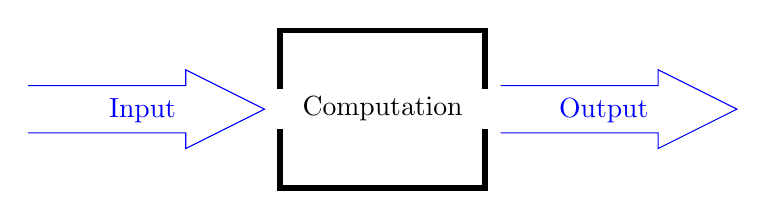
\begin{tikzpicture}
\path[draw][line width=2pt,xscale=1.3] (-1,-0.25) -- (-1,-1)--(1,-1)--(1,-0.25)
			(-1,0.25) -- (-1,1) -- (1,1) -- (1,0.25);
\path (0,0) node{Computation};
\path[draw][color=blue,xshift=-0.5cm] (-4,0.3) -- (-2,0.3) -- (-2,0.5) -- (-1,0) -- (-2,-0.5) -- (-2,-0.3) node[above left]{Input}--(-4,-0.3);
\path[draw][color=blue, xshift=5.5cm] (-4,0.3) -- (-2,0.3) -- (-2,0.5) -- (-1,0) -- (-2,-0.5) -- (-2,-0.3) node[above left]{Output}--(-4,-0.3);
\end{tikzpicture}
\caption{Model of computation.}
\label{fig:model of computation}
\end{figure}

So we have a certain function $f(input)\:=\:output$.


\subsection{Words spaces and alphabet trees}
We begin with the formalization of input and output.

\begin{definition}
An \emph{alphabet} $\abece$ is a finite set of elements called \emph{letters}.
\end{definition}

\begin{definition}
The set $\fslovar:=\{x_1\dots x_n|n\in\N\cup\{0\}, x_i\in\abece \}$ is called the \emph{set of finite words} or \emph{finite dictionary}, and its elements are called \emph{words}.  The element with no letters, written as $\varnothing$, is called the \emph{empty word}. The cartesian product $\abece^n$ is identified with the set of words of lenght $n$.
\end{definition}

\begin{definition}
Let $\word{w}=x_1\dots x_n$ and $\word{u}=y_1\dots y_m$ be words. The \emph{lenght} of $\word{w}$, written as $|\word{w}|$, is $n$. The lenght of the empty word is $0$. The \emph{concatenation} of $\word{w}$ and $\word{u}$, written as $\word{w}\circ \word{u}=\word{w}\word{u}$, is the word $x_1\dots x_n y_1\dots y_m$.
\end{definition}


\begin{example}
Let $\abece=\{0,1\}$. Then $0100\circ 111=0100111$ and $11\circ 0101=110101$.
Let $\abece=\{0,j,2\}$. Then $02j\circ 20j=02j20j$ and $j\circ 2j=j2j$.
\end{example}

\begin{proposition}
$(\fslovar, \circ)$ is a monoid, called the \emph{free monoid on $\abece$}.
\begin{proof}
The operation $\circ$ is associative with $\varnothing$ being an identity element.
\end{proof}
\end{proposition}

Let us define also words of infinite lenght.

\begin{definition}
The \emph{set of infinite words} or the \emph{infinite dictionary} is the set $\infslovar:=\{x_1\dots x_i\dots|x_i\in \abece\}=\abece^{\N\cup\{0\}}$.
\end{definition}

\begin{remark}
Note that if $\word{u}=x_1\dots x_n\in\fslovar$ and $\word{v}=y_1\dots y_i\ldots \in\infslovar$, we can define $\word{u}\circ\word{v}:=x_1\dots x_n y_1\dots y_i\ldots \in\infslovar$.
\end{remark}

\begin{definition}
A word $\word{w}=x_1\dots x_n$ is the \emph{beginning} or the \emph{prefix} of a word $\word{u}\in\fslovar$ (or $\word{u}\in\infslovar$) if $\word{u}=\word{w}\word{v}=x_1\dots x_n \word{v}$ for some $\word{v}\in\fslovar$ (or $\in\infslovar$). In this case we set $\word{v}=\word{u}-\word{w}$.
\end{definition}


\begin{proposition}
Given $A \subseteq\fslovar\cup\infslovar$, the word $\prefix(A)$, the \emph{longest common prefix of all the words from $A$}, is uniquely defined.
\end{proposition}
\begin{proof}
If $A=\{\word{w}\}$ then $\prefix(A)=\{\word{w}\}$ and the proof is finished. Let $|A|>1$. We define $P:=\{\word{p}\in\fslovar\cup\infslovar : \word{p} \text{ is a prefix for every }\word{w}\in A\}$. If $P=\{\varnothing\}$, then $\prefix(A)=\varnothing$ and the proof is finished. Let $P\neq\{\varnothing\}$. If $\word{p}\in P$ is of infinite lenght, then $A=\{\word{p}\}$, against the hypothesis that $|A|>1$. Therefore $P\subseteq \fslovar$. Furthermore if $\word{p_1},\word{p_2}\in P$ such that $|\word{p_1}|\leqslant|\word{p_2}|$, then $\word{p_1}$ is a prefix of $\word{p_2}$, because they are both prefixes for every word in $A$. Consequently, $P\subseteq \abece^k$ for some $k\in \N$, otherwise there would be a sequence of prefixes $(\word{q_n})_{n\in\N}$ in $P$ such that $\lim\limits_{n\rightarrow\infty} |\word{q_n}| =\infty$, and so the word $\word{q}\in \infslovar$ such that the prefix of lenght $n$ of $\word{q}$ is $\word{q_n}$ is an element of $P$, against the hypothesis that $|A|>1$. Let $\bar{k}\in\N$ be the minimum number such that $P\subseteq \abece^\bar{k}$. Then there exists $\word{p_1},\word{p_2}\in P$ of lenght $\bar{k}$. But since $|\word{p_1}|\leqslant|\word{p_2}|$ and $|\word{p_2}|\leqslant|\word{p_1}|$, we have that $\word{p_1}$ is a prefix of $\word{p_2}$ and vice versa, so $\word{p_1}=\word{p_2}$, and $\prefix(A)=\word{p_1}$.
\end{proof}


We can endow the set $\infslovar$ with a metric, and consequently a topology. We treat this construction for the sake of completeness, but it will not be used later in the thesis. 

\begin{definition}
Let $\widetilde\lambda=(\lambda_n)_{n\in\N\cup\{0\}}$ be an arbitrary \obs{decreasing} sequence of \obs{positive} numbers such that $\lim\limits_{n\rightarrow\infty} \lambda_n =0$. We define 
\begin{equation}
d_{\widetilde\lambda}(\word{w_1},\word{w_2})=\left\{
\begin{array}{ll}
      0 \;& \text{if }\word{w}_1=\word{w}_2 \\
      \lambda_n  & \text{if }\word{w}_1\neq\word{w}_2 \\
\end{array} 
\right. 
\label{dist infslovar}
\end{equation} 
on $\infslovar$, where $n=|\prefix(\{\word{w_1},\word{w_2}\})|$ is the lenght of the longest common prefix of the words $\word{w_1}$ and $\word{w_2}$. 
\end{definition}

\begin{proposition}
The function $d_{\widetilde\lambda}$ is a \obs{metric}. 
\end{proposition}
\begin{proof}
The function $d_{\widetilde\lambda}$ is always non-negative, is symmetrical and it can be easily proved that $d_{\widetilde\lambda}(\word{w_1},\word{w_2})=0$ if and only if $\word{w_1}=\word{w_2}$. We prove the triangle inequality. Let $n=|\prefix(\{\word{w_1},\word{w_2}\})|$. Let $\word{w_3}\in\infslovar$. We want to show that \begin{equation*} 
d_{\widetilde\lambda}(\word{w_1},\word{w_2})\leq d_{\widetilde\lambda}(\word{w_1},\word{w_3})+d_{\widetilde\lambda}(\word{w_3},\word{w_2})
\end{equation*}
Denote $p:=|\prefix(\{\word{w_1},\word{w_3}\})|$ and $q:=|\prefix(\{\word{w_3},\word{w_2}\})|$. We need to show that $\lambda_n\leq\lambda_p+\lambda_q$. Suppose that $p=\min\{p,q\}$ (if $q=\min\{p,q\}$ the proof is symmetrical). If $p\leq n$, since $\widetilde\lambda$ is decreasing, we obtain $\lambda_n\leq \lambda_p\leq \lambda_p + \lambda_q$. 
Let us prove that $p\leq n$ through reductio ad absurdum. Suppose that $p>n$. We denote the word $\prefix(\{\word{w_1},\word{w_2}\})$ by $x_1\ldots x_n$, the word $\prefix(\{\word{w_1},\word{w_3}\})$ by $x_1\ldots x_n y_{n+1}\ldots y_p$ and the word $\prefix(\{\word{w_3},\word{w_2}\})$ by $x_1\ldots x_n z_{n+1}\ldots z_p\ldots z_q$. But then $x_1\ldots x_n y_{n+1}\ldots y_p=x_1\ldots x_n z_{n+1}\ldots z_p$ because they are of the same lenght and they are both prefixes of $\word{w_3}$. Consequently the last word, of lenght $p$, is a prefix both of $\word{w_1}$ and $\word{w_2}$. Therefore it is a prefix of $x_1\ldots x_n$, so $p\leq n$, contradicting the assumption that $p> n$.
\end{proof}

Every set $\word{w}\infslovar:=\{\word{wu}|\word{u}\in\infslovar\}$ can be seen as a ball of radius $\lambda_{|\word{w}|}$ with the center in an arbitrary point $\word{wu}\in \word{w}\infslovar$.

\begin{remark}
It is often useful to set $\widetilde\lambda=\left\{
\begin{array}{ll}
      \lambda_n=0 \;& \text{if }n=0 \\
      \lambda_n=\frac{1}{n}  & \text{if }n\in\N \\
\end{array} 
\right.$
\end{remark}

It is useful to represent $\fslovar$ in the form of a tree graph: $\varnothing$ is the root and $\word{v}\in\fslovar$ is a child of $\word{u}\in\fslovar$ \obs{if and only if} $\word{u}=\word{v}x$ for some $x\in \abece$. We call the resulting tree graph a \emph{word tree} on $\abece$. An example is given in \autoref{fig:binary tree}. 

\begin{figure}[H]
\centering
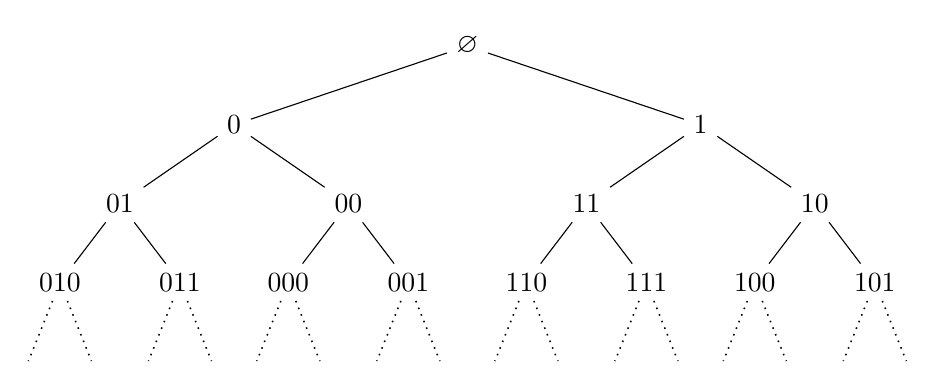
\begin{tikzpicture}[level distance=1cm,
level 1/.style={sibling distance=5.5cm},
level 2/.style={sibling distance=3.5cm, fontscale/.style = small},
level 3/.style={sibling distance=2.3cm},
level 4/.style={sibling distance=0.8cm}]

\node{$\varnothing$} child[left] {node{0}child[right]{node{01} child[right]{node{010} child[dotted,line width=0.2mm] child[dotted,line width=0.2mm]} child[left]{node{011} child[dotted,line width=0.2mm] child[dotted,line width=0.2mm]}	}
child[left]{node{00} child[right]{node{000}child[dotted,line width=0.2mm]child[dotted,line width=0.2mm]} child[left]{node{001}child[dotted,line width=0.2mm]child[dotted,line width=0.2mm]}	}	}
                	child[right] {node{1} child[right]{node{11} child[right]{node{110}child[dotted,line width=0.2mm]child[dotted,line width=0.2mm]} child[left]{node{111}child[dotted,line width=0.2mm]child[dotted,line width=0.2mm]}	} child[left]{node{10} child[right]{node{100}child[dotted,line width=0.2mm]child[dotted,line width=0.2mm]} child[left]{node{101}child[dotted,line width=0.2mm]child[dotted,line width=0.2mm]}	}	};
\end{tikzpicture}
\caption{An example of the word tree $\fslovar$ on $\abece=\{0,1\}$.}
\label{fig:binary tree}
\end{figure}


%\begin{figure}[!h]
%\begin{tikzpicture}[level/.style = {sibling distance=2.5cm, level distance=2cm}]
%
%\node {$\varnothing$}
%    child {  node {$0$}  child[right] { node {$01$} }
%                    	 child[left] { node {$00$} } }
%    child {  node {$1$}  child[right] { node {$11$} }
%                    	 child[left] { node {$10$} }
%             }  ;
%\end{tikzpicture}
%
%\caption{An example of the first three floors of the word tree on $\abece=\{0,1\}$.}
%\label{fig:binary tree}
%\end{figure}

\begin{remark}
We will mostly use the alphabet $\abece=\{0,1\}$.
\end{remark}

The set $\abece^n$ of words of lenght $n$ is called the \obs{the $n$-th floor of $\fslovar$}. Finally we define the notion of an endomorphism of a tree and describe some of its properties.

\begin{definition}\label{def:tree homo}
Let $A$ and $B$ be word trees on some alphabet $\abece$ and $f: A\longrightarrow B$ be a function. It is called a \emph{tree-homomorphism} if it preserves the root and the adjacency of the vertices, i.e.:
\begin{enumerate}
\item If $a\in A$ is the root, $f(a)$ is the root.
\item If $(u,v)$ is an edge of $A$, then $(f(u),f(v))$ is an edge of $B$.
\end{enumerate}
If $A=B$, $f$ is called a \emph{tree-endomorphism}.
If $A=B$ and $f$ is bijective, we call it a \emph{tree-automorphism}.
\end{definition}
It can be verified that all tree-endomorphisms $f:A\longrightarrow A$ form a \obs{semigroup} under the composition of functions, and all the tree-automorphisms $f:A\longrightarrow A$ form its subsemigroup which is also a \obs{group}.

\subsection{Automata and initial automata}
Now we will treat the formal definition of a very specific type of automaton which we need, a \obs{deterministic synchronous automaton}, or \obs{Mealy automaton}, or \obs{transducer}. We will always call it simply an \obs{automaton}, but the reader should know that this is a \obs{very specific} case. Broader class of automata are treated in \cite{4,11}.

\begin{definition}
An \emph{automaton} is a 4-tuple $\auto{A}=\langle\abece,\QQ,\pi,\lambda\rangle$ where:
\begin{itemize}
	\item $\abece$ is an alphabet, usually referred to as the \emph{input} and/or \emph{output alphabet},
	% so here we declare what we put inside and what comes aoutside of the machine
	\item $\QQ$ is a set called the \emph{set of internal states of the automaton},
	\item $\pi:\abece\times\QQ \longrightarrow \QQ $ is a function called the \emph{transition function},
	\item $\lambda:\abece\times\QQ \longrightarrow \abece $ is a function called the \emph{output function}.
\end{itemize}
We say that $\auto{A}$ is a \obs{$|\QQ|$-state} automaton \obs{on $\abece$}.
\end{definition}

This definition explains how an automaton performs the action of transforming an input into an output. %revision reference
We can imagine that for every \obs{input letter} $x$ we plug in the machine, and for every \obs{state} $q$, from which we decide to start, the machine moves to a state $p=\pi(x,q)\in\QQ$ and returns an \obs{output letter} $y=\lambda(x,q)\in\abece$.

\begin{definition}
Given an automaton $\auto{A}=\langle\abece,\QQ,\pi,\lambda\rangle$ we define its \emph{Moore diagram} as the oriented graph $M=(\QQ, \mathcal{E})$ where there is a directed edge from $q_1$ to $q_2$ whenever there exists $x\in \abece$ such that $\pi(x,q_1)=q_2$ and the label assigned to this edge is $x|\lambda(x,q_1)$.
\end{definition}\label{def:moore diagram}

An example of a Moore diagram is given in \autoref{fig:first auto}.
\begin{figure}[h!]
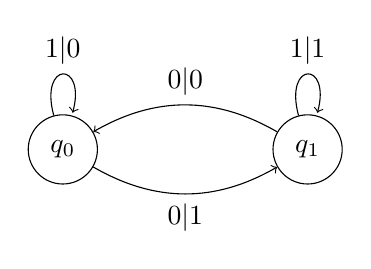
\begin{tikzpicture}
\node[state](q0) at (0,0) {$q_0$};
\node[state, right of=q0, xshift=60] (q1) {$q_1$};
\draw	(q0) edge[below,bend right,-> ] node{$0|1$} (q1)
		(q0) edge[loop above] node{$1|0$} (q0)
		(q1) edge[loop above] node{$1|1$} (q1)
		(q1) edge[above, bend right,-> ] node{$0|0$} (q0);
		
\end{tikzpicture}
\caption{Example of a Moore diagram of a 2-state automaton over the alphabet $\abece=\{0,1\}$}
\label{fig:first auto}
\end{figure}

\begin{remark}
Let $\auto{A}=\langle \abece,\QQ,\pi,\lambda\rangle$ be an automaton and $M=(\QQ, \mathcal{E})$ its Moore diagram. Then $M$ has the following property:
\begin{equation}
\begin{split}
&\forall (x,q)\in \abece\times\QQ \quad\exists! e=(q,p_{(x,q)})\in\mathcal{E} \mtxt{ for some }p=p_{(x,q)}\in\QQ\;s.t.\\
&\mtxt{ the left-hand side of the label of }e\mtxt{ reads ``}x\mtxt{''}.
\end{split}
\label{condition every automaton}
\end{equation}
It follows that if an automaton $\auto{B}=\langle \abece,\QQ_{\auto{B}},\pi_{\auto{B}},\lambda_{\auto{B}}\rangle$ defines the same Moore diagram $M$, then $\QQ_\auto{B}=\QQ$, and for each $(x,q)\in\abece\times\QQ$ we have $\pi_\auto{B}(x,q)=p_{(x,q)}=\pi(x,q)$. Furthermore, for each $x\in\abece$ and for each $q\in\QQ$, $\lambda_\auto{B}(x,q)$ is the right-hand side of the label of the edge $(q,p_{(x,q)})$, i.e., $\lambda_\auto{B}(x,q)=\lambda(x,q)$. So automata are uniquely determined by their Moore diagrams. 
\end{remark}

\begin{example}
In \autoref{fig:first auto}, given the input $\word{w}=0$ and the state $q=q_0$, we have $\pi(\word{w},q)=q_1$ and $\lambda(\word{w},q)=1$. If $\word{w}=1$ and $q=q_1$, then $\pi(\word{w},q)=q_1$ and $\lambda(\word{w},q)=1$.
\end{example}

\begin{definition}
We recursively extend the domain of $\pi$ and $\lambda$ from single letters in $\abece$ to \obs{words} in $\fslovar$. We define:
\begin{itemize}
	\item $\PI:\fslovar \times \QQ\longrightarrow \QQ :$ 
	$$\PI(\varnothing,q)=q,$$ $$\PI(x \word{w},q)=\PI(\word{w},\PI(x,q)).$$
	\item $\LAMBDA:\fslovar \times \QQ\longrightarrow \fslovar :$
	$$\LAMBDA(\varnothing,q)=\varnothing,$$ $$\LAMBDA(x \word{w},q)=\LAMBDA(x,q)\LAMBDA(\word{w},\PI(x,q)).$$
\end{itemize}
\label{def:extended lambda pi}
\end{definition}

\begin{remark}
Definition \autoref{def:extended lambda pi} is equivalent to:
$$\PI(\word{w} x,q)=\PI(x,\PI(\word{w},q))$$ and
$$\LAMBDA(\word{w} x,q)=\LAMBDA(\word{w},q) \LAMBDA(x,\PI(\word{w},q)),$$ respectively.
\end{remark}

\begin{example}
We can compute $\PI$ and $\LAMBDA$ following the arrows on the Moore diagram of an automaton, and then making the composition of the single right-hand side of the labels. In \autoref{fig:first auto}, given the input $\word{w}=0000$ and the state $q=q_0$, we have $\PI(q,\word{w})=q_0$ and $\LAMBDA(q,\word{w})=1010$. If $\word{w}=110$ and $q=q_1$, we have $\PI(q,\word{w})=q_0$ and $\LAMBDA(q,\word{w})=110$.
\end{example}

To effectively make an automaton a word-transducer we need to specify an initial state. For example, in \autoref{fig:first auto} to get an output we need to feed the machine both with an input $x$ and a state $q$. So let us fix $q\in\QQ$.

\begin{definition}
If an  automaton $\auto{A}$ has a fixed state $q_0$, we call it an \emph{initial automaton with the initial state $q_0$} and we write it as $\auto{A}_{q_0}$. Each $\auto{A}_{q_0}$ naturally defines the map $\LAMBDA_{q_0}:\fslovar\longrightarrow\fslovar$ with $\LAMBDA_{q_0}(\word{w}):=\LAMBDA(\word{w},q_0)$, called the \emph{action of the automaton $\auto{A}_{q_0}$}. Two \obs{initial automata} are said to be \emph{equivalent} if they define the same actions.
\end{definition}

In general to prove that two initial automata are equivalent is not trivial.

\begin{proposition}\label{prop:lenght-preserving}
The action $\LAMBDA_{q_0}$ of an initial automaton preserves the lenght of words, i.e., $|\LAMBDA_{q_0}(\word{w})|=|\word{w}|$.
\end{proposition}
\begin{proof}
We verify the statement by induction on $n=|\word{w}|$.

\emph{Case $n=0$}: We defined $\LAMBDA_{q_0}(\varnothing)=\LAMBDA(\varnothing,q_0)=\varnothing$, and $|\varnothing|=|\LAMBDA_{q_0}(\varnothing)|=0$.

\emph{Case $n\Rightarrow n+1$}: Let $|\LAMBDA_{q_0}(\word{w})|=|\word{w}|=n$ for every $\word{w}\in\abece^n$. Following Definition \autoref{def:extended lambda pi} we have $|\LAMBDA_{q_0}(\word{w}x)|=|\LAMBDA_{q_0}(\word{w})\LAMBDA_{\PI(\word{w},q_0)}(x)|=|\LAMBDA_{q_0}(\word{w})|+|\LAMBDA_{\PI(\word{w},q_0)}(x)|=n+1$.
\end{proof}

\begin{remark}
Given an initial automaton $\auto{A}_{q_0}$, we can define the \obs{infinite action $\LAMBDA_{q_0}:\infslovar\longrightarrow\infslovar$} by similar recursive formulas, and we can consequently declare that two initial automata are \obs{$\omega$-equivalent} if they determine the same infinite action. Two automata are equivalent \obs{if and only if} they are $\omega$-equivalent (Proposition 2.3 and Subsection 3.1 in \cite{5}).
\label{equivalence of automata}
\end{remark}

\begin{example}
In \autoref{fig:equivalent initial automata} we present the Moore diagrams of two equivalent initial automata.
\end{example}

\begin{remark}
An initial automaton is usually drawn depicting the initial state with a double circle around the respective vertex (\autoref{fig:equivalent initial automata}).
\end{remark}

Let us stress once again that an automaton does not define any function, till we do not fix a state $q_0$.
\begin{figure}[h]
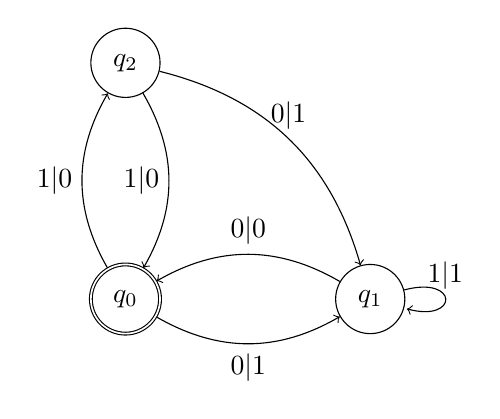
\begin{tikzpicture}
\node[accepting,state](q0) at (0,0) {$q_0$};
\node[state, right of=q0, xshift=60] (q1) {$q_1$};
\node[state](q2) at (0,3) {$q_2$};

\draw	(q0) edge[below,bend right,-> ] node{$0|1$} (q1)
		(q0) edge[left, bend left, -> ] node{$1|0$} (q2)
		(q1) edge[loop right,above] node{$1|1$} (q2)
		(q1) edge[above, bend right,-> ] node{$0|0$} (q0)
		(q2) edge[left, bend left, -> ] node{$1|0$} (q0)
		(q2) edge[above,bend left,->] node{$0|1$} (q1);
		
\end{tikzpicture}
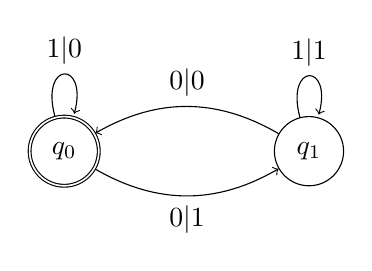
\begin{tikzpicture}
\node[accepting, state](q0) at (0,0) {$q_0$};
\node[state, right of=q0, xshift=60] (q1) {$q_1$};
\draw	(q0) edge[below,bend right,-> ] node{$0|1$} (q1)
		(q0) edge[loop above] node{$1|0$} (q0)
		(q1) edge[loop above] node{$1|1$} (q1)
		(q1) edge[above, bend right,-> ] node{$0|0$} (q0);
		
\end{tikzpicture}
\caption{Two different initial automata which describe the same action. The double circle around $q_0$ tells us $q_0$ is the initial state.}
\label{fig:equivalent initial automata}
\end{figure}

\smallskip
\section{The algebraic structures defined by automata}
Here we will show how automata can define algebraic structures and how certain synchronous automatic transformations can be characterised.

\begin{definition}\label{def:aut composition}
Given automata $\auto{A}_1=\langle \abece,\QQ^{\auto{A}_1},\pi^{\auto{A}_1},\lambda^{\auto{A}_1}\rangle$ and $\auto{A}_2=\langle  \abece,\QQ^{\auto{A}_2},\pi^{\auto{A}_2},\lambda^{\auto{A}_2}\rangle$, we define their \obs{composition} $\auto{B}:=\auto{A}_1*\auto{A}_2=\:\langle \abece,\QQ^{\auto{A}_1}\times\QQ^{\auto{A}_2},\pi,\lambda\rangle$ with $\pi$ and $\lambda$ defined as follows:
\begin{itemize}
\item $\pi(x,(s_1,s_2))=(\pi^{\auto{A}_1}(x,s_1),\pi^{\auto{A}_2}(\lambda^{\auto{A}_1}(x,s_1),s_2))$,
\item $\lambda(x,(s_1,s_2))=\lambda^{\auto{A}_2}(\lambda^{\auto{A}_1}(x,s_1),s_2)$,
\end{itemize}
where $x\in \abece$ and $(s_1,s_2)\in\QQ^{\auto{A}_1}\times\QQ^{\auto{A}_2}=\QQ$.
\end{definition}


\begin{proposition}\label{obs:first obs on compostion}
Let $\auto{A}_1,\auto{A}_2$ be as in Definition \ref{def:aut composition} and let $(\auto{A}_1)_{q_1}$ and $(\auto{A}_2)_{q_2}$ be initial automata for some $q_1\in\QQ^{\auto{A}_1},q_2\in\QQ^{\auto{A}_2}$. Then for every word $\word{w}\in\fslovar$ the following holds: 
$$ (\LAMBDA^{\auto{A}_2}_{q_2} \circ \LAMBDA^{\auto{A}_1}_{q_1})(\word{w}) = \LAMBDA^{\auto{A}_1*\auto{A}_2}_{(q_1,q_2)}(\word{w}).$$
\end{proposition}
\begin{proof}
If $\word{w}=\varnothing$ the coclusion is trivial. We proceed by induction on $n=|\word{w}|$.

\emph{Case $n=1$}: Let $x\in\abece$. Then
\begin{align*}
(\LAMBDA_{q_2}^{\auto{A}_2}\circ\LAMBDA_{q_1}^{\auto{A}_1})(x)=&
\LAMBDA_{q_2}^{\auto{A}_2}(\LAMBDA_{q_1}^{\auto{A}_1}(x))=
\LAMBDA_{q_2}^{\auto{A}_2}(\LAMBDA^{\auto{A}_1}(x,q_1))=
\LAMBDA^{\auto{A}_2}(\LAMBDA^{\auto{A}_1}(x,q_1),q_2)\\=&
\lambda^{\auto{A}_2}(\lambda^{\auto{A}_1}(x,q_1),q_2)=
\lambda^{\auto{A}_1*\auto{A}_2}(x,(q_1,q_2))\\=&
\lambda^{\auto{A}_1*\auto{A}_2}_{(q_1,q_2)}(x)=
\LAMBDA^{\auto{A}_1*\auto{A}_2}_{(q_1,q_2)}(x)
\end{align*}

\emph{Case $n\Rightarrow n+1$}: Let us suppose that $ (\LAMBDA^{\auto{A}_2}_{q_2} \circ \LAMBDA^{\auto{A}_1}_{q_1})(\word{w}) = \LAMBDA^{\auto{A}_1*\auto{A}_2}_{(q_1,q_2)}(\word{w})$ is valid for every $\word{w}\in\abece^n$. Let $x\in\abece$ and $\word{w}\in\abece^n$. Then 
\begin{align*}
(\LAMBDA_{q_2}^{\auto{A}_2}\circ\LAMBDA_{q_1}^{\auto{A}_1})(x\word{w})=&
\LAMBDA_{q_2}^{\auto{A}_2}\textcolor{red}{(}\LAMBDA_{q_1}^{\auto{A}_1}(x\word{w})\textcolor{red}{)}=
\LAMBDA_{q_2}^{\auto{A}_2}\textcolor{red}{(}\LAMBDA^{\auto{A}_1}(x\word{w},{q_1})\textcolor{red}{)}\\
=&\LAMBDA_{q_2}^{\auto{A}_2}\textcolor{red}{(}		\LAMBDA^{\auto{A}_1}(x,{q_1}) 	\LAMBDA^{\auto{A}_1}(\word{w},\pi^{\auto{A}_1}(x,{q_1})	\textcolor{red}{)}\\=&
\LAMBDA^{\auto{A}_2}\textcolor{red}{(}	\underbrace{\LAMBDA^{\auto{A}_1}(x,{q_1})} 	\underbrace{\LAMBDA^{\auto{A}_1}(\word{w},\pi^{\auto{A}_1}(x,{q_1})})	,q_2\textcolor{red}{)}\\=&
\LAMBDA^{\auto{A}_2}\textcolor{red}{(}	\underbrace{\LAMBDA^{\auto{A}_1}(x,{q_1})},	q_2\textcolor{red}{)} 	\LAMBDA^{\auto{A}_2}\textcolor{red}{(}\underbrace{\LAMBDA^{\auto{A}_1}(\word{w},\pi^{\auto{A}_1}(x,{q_1}))}	,\pi^{\auto{A}_2}(\LAMBDA^{\auto{A}_1}(x,{q_1}),q_2)\textcolor{red}{)}\\=&
\LAMBDA^{\auto{A}_2}_{q_2}\textcolor{red}{(}	\underbrace{\LAMBDA^{\auto{A}_1}_{q_1}(x)}\textcolor{red}{)} 	\LAMBDA^{\auto{A}_2}_{\pi^{\auto{A}_2}(\LAMBDA^{\auto{A}_1}(x,{q_1}),q_2)}\textcolor{red}{(}\underbrace{\LAMBDA^{\auto{A}_1}_{\pi^{\auto{A}_1}(x,{q_1})}(\word{w})}\textcolor{red}{)}.
\end{align*}
Since the lenght of both $x$ and $\word{w}$ is $\leqslant n$ we have that 
\begin{align*}
\LAMBDA^{\auto{A}_2}_{q_2}\textcolor{red}{(}	\LAMBDA^{\auto{A}_1}_{q_1}(x)\textcolor{red}{)}&=\LAMBDA^{\auto{A}_1*\auto{A}_2}_{(q_1,q_2)}(x)\\
\LAMBDA^{\auto{A}_2}_{\pi^{\auto{A}_2}(\LAMBDA^{\auto{A}_1}(x,{q_1}),q_2)}\textcolor{red}{(}\LAMBDA^{\auto{A}_1}_{\pi^{\auto{A}_1}(x,{q_1})}(\word{w})\textcolor{red}{)}&=\LAMBDA^{\auto{A}_1*\auto{A}_2}_{(\pi^{\auto{A}_1}(x,{q_1}),\pi^{\auto{A}_2}(\LAMBDA^{\auto{A}_1}(x,{q_1}),q_2))}(\word{w})\\&=\LAMBDA^{\auto{A}_1*\auto{A}_2}_{\pi^{\auto{A}_1*\auto{A}_2}(x,{(q_1,q_2)})}(\word{w})
\end{align*} 
and therefore
\begin{align*}
\underbrace{\LAMBDA^{\auto{A}_2}_{q_2}\textcolor{red}{(}	\LAMBDA^{\auto{A}_1}_{q_1}(x)\textcolor{red}{)}} 	\underbrace{\LAMBDA^{\auto{A}_2}_{\pi^{\auto{A}_2}(\LAMBDA^{\auto{A}_1}(x,{q_1}),q_2)}\textcolor{red}{(}\LAMBDA^{\auto{A}_1}_{\pi^{\auto{A}_1}(x,{q_1})}(\word{w})\textcolor{red}{)}}&=
\underbrace{\LAMBDA^{\auto{A}_1*\auto{A}_2}_{(q_1,q_2)}(x)}\underbrace{\LAMBDA^{\auto{A}_1*\auto{A}_2}_{\pi^{\auto{A}_1*\auto{A}_2}(x,{(q_1,q_2)})}(\word{w})}\\&=\LAMBDA^{\auto{A}_1*\auto{A}_2}_{(q_1,q_2)}(x\word{w}).
\end{align*}
And so the proof is finished.
\end{proof}


\begin{remark}
Proposition \ref{obs:first obs on compostion} means that the operation $*$ on the set of \obs{automata} gives rise to an operation $*'$ on the set of \obs{initial automata} defined as $(\auto{A}_1)_{q_1}*'(\auto{A}_2)_{q_2}:=(\auto{A}_1*\auto{A}_2)_{(q_1,q_2)}$. With the operation $*'$ the set of all initial automata on an alphabet $\abece$ becomes a \obs{semigroup}.
\end{remark}

\begin{figure}[H]
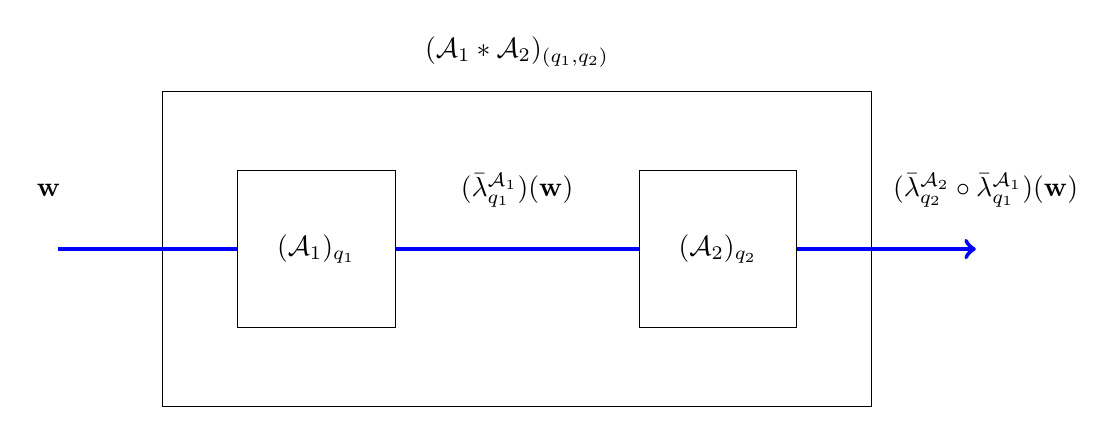
\begin{tikzpicture}[xscale=0.85,xshift=-0.2cm]
\node[draw,rectangle,minimum width=2cm, minimum height = 2cm] (auto1) at (-3cm,0) {$(\auto{A}_1)_{q_1}$};
\node (input) at (-7cm,0) {};
\node[above of=input,yshift=-0.25cm] {$\word{w}$};
\node[draw,rectangle,minimum width=2cm, minimum height = 2cm] (auto2) at (3cm,0) {$(\auto{A}_2)_{q_2}$};
\node (output) at (7cm,0) {};
\node[above of=output, yshift=-0.25cm] {$(\LAMBDA^{\auto{A}_2}_{q_2} \circ \LAMBDA^{\auto{A}_1}_{q_1})(\word{w})$};
\node[draw,rectangle,minimum width=9cm, minimum height = 4cm] (auto1*auto2) at (0,0){};
\node[above of=auto1*auto2,yshift=-0.25cm] (auto1*auto2) {$(\LAMBDA^{\auto{A}_1}_{q_1})(\word{w})$};
\node at (0,2.5cm) {$(\auto{A}_1*\auto{A}_2)_{(q_1,q_2)}$};

\path[line width=1.6pt,draw,-> ,color=blue] (input)-> (auto1)-> (auto2)-> (output);
\end{tikzpicture}
\caption{Concept of composition of initial automata.}
\label{fig:composition of automata}
\end{figure}

\smallskip
\subsection{Synchronous automatic transformations}
In this section, given an action of an initial automaton, we describe and study its properties.

\begin{definition}
A transformation on $\fslovar$(i.e., a function $f:\fslovar\longrightarrow\fslovar$) is called \emph{finite synchronous automatic} if it is the (finite) action of some initial automaton $\auto{A}_{q_0}$, i.e., if $f=\LAMBDA_{q_0}$.
\end{definition}

\begin{definition}
A transformation on $\infslovar$(i.e., a function $f:\infslovar\longrightarrow\infslovar$) is called \emph{infinite synchronous automatic} if it is the infinite action of some initial automaton. 
\end{definition}


\begin{proposition}
The finite synchronous automatic transformations form a semigroup denoted by $\semisynaut(\abece)$.
\end{proposition}
\begin{proof}
This arises from Proposition \autoref{obs:first obs on compostion}. Let $f_1=\LAMBDA^{\auto{A}_1}_{q_1}$ and $f_2=\LAMBDA^{\auto{A}_2}_{q_2}$ be the actions of two initial automata $(\auto{A}_1)_{q_1}$ and $(\auto{A}_2)_{q_2}$ respectively. We have seen that 
$$f_2 \circ f_1 = \LAMBDA^{\auto{A}_2}_{q_2} \circ \LAMBDA^{\auto{A}_1}_{q_1} = \LAMBDA^{\auto{A}_1*\auto{A}_2}_{(q_1,q_2)},$$
hence $f_2 \circ f_1$ is synchronous automatic. Therefore $\semisynaut(\abece)$ is closed under composition of functions and consequently it is a semigroup.
\end{proof}

Now we provide an important characterization of synchronous automatic transformations:

\begin{proposition}\label{prop:equivalence tree-morph and semisynaut}
A transformation $f:\fslovar\longrightarrow\fslovar$ is synchronous automatic \obs{if and only if} $f$ is a tree-endomorphism on $\fslovar$.
\end{proposition}
\begin{proof}
\emph{$(\Rightarrow)$}: Since $f$ is synchronous automatic, there is an action $\LAMBDA_{q_0}$ of some initial automaton such that $f=\LAMBDA_{q_0}$. We need to show that $\LAMBDA_{q_0}$ (1) preserves the root and (2) preserves the adjacency of vertices. 
By the definition $f(\varnothing)=\LAMBDA_{q_0}(\varnothing)=\varnothing$, thus (1) holds. 
Now we prove (2): if $\word{v}\text{ is a child of }\word{w}$ (i.e., $\word{v}=\word{w}x\text{ for some }x\in\abece$), we show that $f(\word{v})\text{ is a child of }f(\word{w})$ (i.e., $f(\word{v})=f(\word{w})y\text{ for some }y\in\abece$). We have:
\begin{align*}
f(\word{v})&=f(\word{w}x)=\LAMBDA_{q_0}(\word{w}x)=\LAMBDA(\word{w}x,q_0)
\\
&=\LAMBDA(\word{w},q_0)\LAMBDA(x,\PI(\word{w},q_0))=f(\word{w})\LAMBDA(x,\PI(\word{w},q_0)).
\end{align*}
But $|\LAMBDA(x,\PI(\word{w},q_0))|=1$ because every action is lenght-preserving, thus $y=\LAMBDA(x,\PI(\word{w},q_0))\in\abece$, so $f(\word{v})=f(\word{w}x)=f(\word{w})y$, hence (2) holds as well.

\smallskip

\emph{$(\Leftarrow)$}: Let $f:\fslovar\longrightarrow\fslovar$ be a tree-endomorphism. We must find an initial automaton such that its action is equal to $f$. We define $\auto{A}=\langle \abece,\QQ,\pi,\lambda\rangle :=\langle \abece,\fslovar,\pi,\lambda\rangle$ ($\QQ=\fslovar$ is \obs{infinite}) with $\pi(x,\word{q}):=\word{q}x$ and $\lambda(x,\word{q}):=f(\word{q}x)-f(\word{q})$. 

First we show that the output function $\lambda$ is well defined, i.e., the subtraction $f(\word{q}x)-f(\word{q})$ is well defined. Because $f$ is a tree-endomorphism, $f(\word{q}x)$ is a child of $f(\word{q})$. 
Now we check if $\LAMBDA_{\varnothing}$, the action of $\auto{A}_{\varnothing}$, corresponds to the function $f$. We verify that $\LAMBDA_{\varnothing}(\word{w})=f(\word{w})$ by induction on $n=|\word{w}|$.

\emph{Case $n=0$}: We have $\LAMBDA(\varnothing,\varnothing)=\varnothing=f(\varnothing)$. 

\emph{Case $n\Rightarrow n+1$}: Given $\word{w}\in\fslovar\setminus\{\varnothing\}$, it can be written as $\word{v}x$, with $\word{v}\in\fslovar$ and $x\in\abece$. 
Then $\LAMBDA(\word{v}x,\varnothing)=\LAMBDA(\word{v},\varnothing)\LAMBDA(x,\PI(\word{v},\varnothing))=f(\word{v})\LAMBDA(x,\word{v})=f(\word{v})[f(\word{v}x)-f(\word{v})] $ which finishes the proof.
\end{proof}

\begin{proposition}\label{prop:tree-endomorph preserve lenght}
If $f$ is a tree-endomorphism on $\fslovar$, then $f(\abece^n)\subseteq \abece^n$. In particular, if $f$ is a tree-automorphism, then $f(\abece^n)=\abece^n$, i.e., it is a permutation on $\abece^n$.
\end{proposition}
\begin{proof}
It follows from Proposition \autoref{prop:lenght-preserving} and Proposition \autoref{prop:equivalence tree-morph and semisynaut}. The second point arises from the bijectivity of the tree-automorphism $f$.
\end{proof}

Proposition \autoref{prop:tree-endomorph preserve lenght} provides a graph perspective on the lenght-preserving condition of actions of automata.

\begin{proposition}\label{prop:tree-restriction}
Let $\word{vw}\in\fslovar$ and $g$ a tree-endomorphism. Then $g(\word{v})$ is a prefix of $g(\word{vw})$. 
\end{proposition}
\begin{proof}
We prove it by induction on $|\word{w}|=n$.

\emph{Case $n=0$}: We have that $g(\word{vw})=g(\word{v})$, which is a prefix of itself.

\emph{Case $n\Rightarrow n+1$}: Let us suppose $g(\word{v})$ is a prefix of $g(\word{vw})$ for every $\word{w}\in\abece^n$. We have that $g(\word{vw}x)=g(\word{vw})y$ for some $y\in\abece$. Since $g(\word{v})$ is a prefix of $g(\word{vw})$ which is a prefix of $g(\word{vw})y=g(\word{vw}x)$, we have that $g(\word{v})$ is a prefix of $g(\word{vw}x)$, and thus the proof is finished.
\end{proof}

\begin{definition}
Let $g:\fslovar\longrightarrow\fslovar$ be a \obs{tree-endomorphism} and $\word{v}\in\fslovar$. We define the \emph{restriction of $g$ in $\word{v}$} as the function $g|_{\word{v}}:\fslovar\longrightarrow\fslovar$ such that:
\label{def:tree-restriction}
\begin{equation}\label{eq:restriction}
g(\word{vw})=g(\word{v})g|_{\word{v}}(\word{w}).
\end{equation}
\end{definition}

\begin{remark}
Equation \eqref{eq:restriction} is well defined because, as proved in Proposition \autoref{prop:tree-restriction}, $g(\word{v})$ is a prefix of $g(\word{vw})$.
\end{remark}

\begin{proposition}
Let $g$,$\word{v}$ and $g|_{\word{v}}$ be as in Definition \autoref{def:tree-restriction}, then $g|_{\word{v}}(\word{w})=g(\word{vw})-g(\word{v})$. Furthermore, $g|_{\word{v}}$ is a tree-endomorphism.
\end{proposition}
\begin{proof}
The first point is a direct consequence of Proposition \autoref{prop:tree-restriction}. Let us prove the second point. We have that $g|_{\word{v}}(\varnothing)=g(\word{v})-g(\word{v})=\varnothing$, so $g|_{\word{v}}$ preserves the root. Furthermore, if $x\in\abece$, then $g|_{\word{v}}(\word{w}x)=g(\word{vw}x)-g(\word{v})=g(\word{vw})y-g(\word{v})$ for some $y\in\abece$ (because $g$ is a tree-endomorphism), and finally $g(\word{vw})y-g(\word{v})=(g(\word{vw})-g(\word{v}))y=g|_{\word{v}}(\word{w})y$, and therefore $g|_{\word{v}}$ is a tree-endomorphism.
\end{proof}

We give a description of the restriction $g_{|_\word{v}}$ in terms of automata.

\begin{proposition}
If $\LAMBDA_{q_0}:\fslovar\longrightarrow\fslovar$ is the action of $\auto{A}_{q_0}$, then, for every $\word{v}\in\fslovar$, the action of $\auto{A}_{\PI(\word{v},q_0)}$ is given by $(\LAMBDA_{q_0})|_{\word{v}}=\LAMBDA_{\PI(\word{v},q_0)}$, i.e., the restriction of $\LAMBDA_{q_0}$ in $\word{v}$.
\label{prop:restr on automata}
\end{proposition}
\begin{proof}
Given $\word{v},\word{w}\in\fslovar$ we can easily prove by induction on $n=|\word{w}|$ that $g(\word{vw}):=\LAMBDA_{q_0}(\word{vw})=\LAMBDA_{q_0}(\word{v})\LAMBDA_{\PI(\word{v},q_0)}(\word{w})=g(\word{v})\LAMBDA_{\PI(\word{v},q_0)}(\word{w})$, consequently $g|_\word{v}=\LAMBDA_{\PI(\word{v},q_0)}$.
\end{proof}

\smallskip
\subsection{Groups generated by automata}

\begin{definition}
Given an initial automaton $\auto{A}_{q_0}$, a state $q$ is called \emph{accessible} if there exists a word $\word{w}\in\fslovar$ such that $\PI(\word{w},q_0)=q$. We can also say that $q$ \emph{ is accessible with respect to} $q_0$ or \emph{from} $q_0$.
\end{definition}

This means that in the Moore diagram there is a path from $q_0$ to $q$.

\begin{definition}
An initial automaton $\auto{A}_{q_0}$ is called \emph{accessible} if each $q\in\QQ$ is accessible with respect to $q_0$. An automaton is called \emph{accessible} if each initial automaton defined by it is accessible.
\end{definition}

\begin{proposition}
Given an automaton $\auto{A}=\langle \abece,\QQ,\pi,\lambda\rangle$ and a state $q_0\in\QQ$, $\LAMBDA_{q_0}$ is an invertible function \obs{if and only if} for every accessible state $q\in\QQ$ (respect to $q_0$) the function $\lambda_q:\abece\longrightarrow\abece$ is invertible.
\end{proposition}

\begin{proof}
\emph{($\Rightarrow$)}: Suppose that $\LAMBDA_{q_0}$ is an invertible function. Let us take an accessible state $q\in\QQ$ and a word $\word{w}$ such that $\PI_{q_0}(\word{w})=q$. We check that $\lambda_q$ is injective. Let $x\neq y$. From the converse we suppose that $\lambda_q(x)=\lambda_q(y)$. We would then have that 
$$\LAMBDA_{q_0}(\word{w}x)=\LAMBDA_{q_0}(\word{w})\underbrace{\LAMBDA_{\PI(\word{w},q_0)}(x)}=\LAMBDA_{q_0}(\word{w})\underbrace{\lambda_{q}(x)}=\LAMBDA_{q_0}(\word{w})\lambda_{q}(y)=\LAMBDA_{q_0}(\word{w}y).$$
Consequently, we would lose the injectivity of $\LAMBDA_{q_0}$, contradicting the hypothesis of its invertibility. Analogously we can see that $\lambda_q$ is surjective: let us take a word $\word{w}\in\fslovar$ such that $\PI(\word{w},q_0)=q$ and $y\in\abece$. We search an $x\in\abece$ such that $\lambda_q(x)=y$. Since $\LAMBDA_{q_0}$ is invertible and synchronous automatic, the word $\LAMBDA_{q_0}(\word{w})y$ has a unique preimage, and it is of the form $\word{w}x$ for some $x$. Therefore: $\LAMBDA_{q_0}(\word{w})y=\LAMBDA_{q_0}(\word{w}x)=\LAMBDA_{q_0}(\word{w})\lambda_q(x)$.

\emph{($\Leftarrow$)}: The transition function moves necessarily to an accessible state $q$ for each $\word{w}\in\fslovar$. We know that $\lambda_p:\abece\longrightarrow\abece$ is invertible for each accessible $p$, including all the states on the path to $q$. 
Now we will prove that $\LAMBDA_{q_0}$ is invertible on $\abece^n$ by induction on $n$, consequently it will be invertible on $\bigcup_{n\in\N\cup\{0\}} \abece^n=\fslovar$.

\emph{Case $n=1$}: On $\abece$ we have $\LAMBDA_{q_0}=\lambda_{q_0}$, therefore $\LAMBDA_{q_0}$ is invertible by the hypothesis.

\emph{Case $n\Rightarrow n+1$}: Let us suppose that $\LAMBDA_{q_0}$ is invertible on $\abece^n$. If $\word{v}\in\abece^{n+1}$ then $\word{v}=\word{w}x\in\abece^n\times\abece$ with $|\word{w}|=n$. Thus $\LAMBDA_{q_0}(\word{v})=\LAMBDA_{q_0}(\word{w}x)=\LAMBDA_{q_0}(\word{w})\LAMBDA_{\PI(\word{w},q_0)}(x)=\LAMBDA_{q_0}(\word{w})\lambda_p(x)$ for some $p$. 
We observe now that if we change $\word{w}$ or $x$, we obtain a different image with respect to $\LAMBDA_{q_0}$ on $\abece^n$ and with respect to $\lambda_{q_0}$ on $\abece$ (injectivity). Furthermore, if we search for the preimage of a word $\word{\bar{w}}\bar{x}\in\abece^{n+1}$, we know that there exists a preimage $\word{w}$ of $\word{\bar{w}}$ through $\LAMBDA_{q_0}$ and a preimage $x$ of $\bar{x}$ with respect to $\lambda_{\PI(\word{w},q_0)}$. If we glue them together, we obtain:
$$\LAMBDA_{q_0}(\word{w}x)=\LAMBDA_{q_0}(\word{w})\lambda_{\PI(\word{w},q_0)}(x)=\word{\bar{w}}\bar{x}.$$
So surjectivity of $\LAMBDA_{q_0}$ is proven.
\end{proof}


\begin{proposition}
The set $\synaut(\abece)$ of all \obs{bijective} synchronous automatic transformations on an alphabet $\abece$ is a group with respect to the composition operation. Furthermore, it is isomorphic to $\aut_{tree}(\fslovar)$, the group of all tree-automorphisms of $\fslovar$.
\label{prop:aut_tree isomorph to synaut}
\end{proposition}
\begin{proof}
The set $\synaut(\abece)$ consists of all bijective elements of $\semisynaut(\abece)$, hence it is a group.
\end{proof}

\begin{definition}
An initial automaton $\auto{A}_{q_0}$ is called \emph{invertible} if its action is invertible. An automaton $\auto{A}$ is called \emph{invertible} if $\auto{A}_{q_0}$ is invertible for each $q_0\in\QQ$.
\end{definition}

\begin{remark}
We introduce a different notation for Moore diagrams. Let $q,p$ be vertices of a Moore diagram and $q\longrightarrow p$ an edge between them. Recalling Definition \autoref{def:moore diagram}, this means there exist $x,y\in\abece$ such that $\pi(x,q)=p$ and $\lambda(x,q)=y$. Then we label the arrow from $q$ to $p$ by the letter $x$ and the vertex $q$ by the function $\lambda_{q}=\lambda(\cdot,q):\abece\longrightarrow\abece$. See \autoref{fig:diff notations} for an example.
\end{remark}

\begin{figure}[H]
\begin{center}
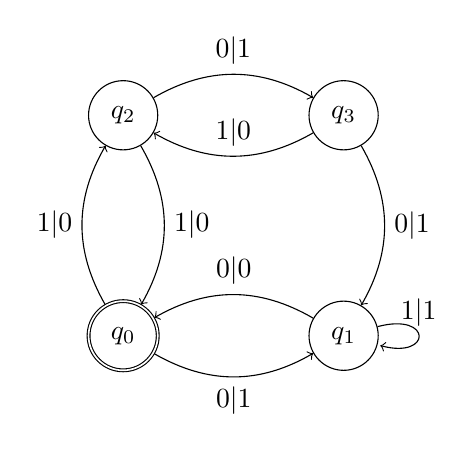
\begin{tikzpicture}[scale=0.7]
\node[accepting,state](q0) at (0,0) {$q_0$};
\node[state](q1) at (4,0) {$q_1$};
\node[state](q2) at (0,4) {$q_2$};
\node[state](q3) at (4,4) {$q_3$};

\draw	(q0) edge[below,bend right,-> ] node{$0|1$} (q1)
		(q0) edge[left, bend left, -> ] node{$1|0$} (q2)
		(q1) edge[loop right,above] node{$1|1$} (q2)
		(q1) edge[above, bend right,-> ] node{$0|0$} (q0)
		(q2) edge[right, bend left, -> ] node{$1|0$} (q0)
		(q2) edge[above,bend left,-> ] node{$0|1$} (q3)
		
		(q3) edge[right,bend left,-> ] node{$0|1$} (q1)
		(q3) edge[above,bend left,-> ] node{$1|0$} (q2)
		;
		
\end{tikzpicture}
\quad
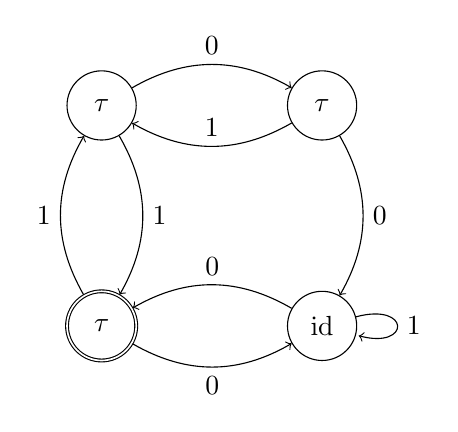
\begin{tikzpicture}[scale=0.7]
\node[accepting,state](q0) at (0,0) {$\tau$};
\node[state](q1) at (4,0) {$\id$};
\node[state](q2) at (0,4) {$\tau$};
\node[state](q3) at (4,4) {$\tau$};

\draw	(q0) edge[below,bend right,-> ] node{$0$} (q1)
		(q0) edge[left, bend left, -> ] node{$1$} (q2)
		(q1) edge[loop right,right] node{$1$} (q2)
		(q1) edge[above, bend right,-> ] node{$0$} (q0)
		(q2) edge[right, bend left, -> ] node{$1$} (q0)
		(q2) edge[above,bend left,-> ] node{$0$} (q3)
		(q3) edge[right,bend left,-> ] node{$0$} (q1)
		(q3) edge[above,bend left,-> ] node{$1$} (q2)
		;
		
\end{tikzpicture}
\end{center}
\caption{An example of the same initial automaton represented in two different ways. In the right figure $\tau, \id\in\symm_2:=\symm(\{0,1\})$, where, $\tau=\lambda_{q_0}=\lambda_{q_2}=\lambda_{q_3}$ inverts the elements in $\{0,1\}$ and $\id=\lambda_{q_1}$ leaves them unchanged.}
\label{fig:diff notations}
\end{figure}

\begin{definition}
Given an automaton $\auto{A}=\langle \abece, \QQ, \pi, \lambda\rangle$ we can define $|\QQ|$ initial automata, which define $|\QQ|$ actions $\LAMBDA_{q}$ on $\fslovar$ inside $\semisynaut(\abece)$. By the \emph{semigroup generated by $\auto{A}$} we mean the subsemigroup $H(\auto{A})$ of $\semisynaut(\abece)$ generated by all the actions $\LAMBDA_{q}$ with $q\in\QQ$:
$$H(\auto{A})=\langle \{\LAMBDA_q:\fslovar\longrightarrow\fslovar | q\in\QQ\}\rangle, $$
where, for a set $S$, $\langle S\rangle$ means the semigroup generated by the elements of $S$, i.e., the smallest subsemigroup of $\semisynaut(\abece)$ which contains all the elements of $S$.
\end{definition}

\begin{remark}
If $\auto{A}$ is invertible then $H(\auto{A})$ is the \emph{group generated by $\auto{A}$}, and we have that $H(\auto{A}) \subseteq \synaut(\abece)$.
\end{remark}

\begin{remark}
From now on by an automaton and by an initial automaton we mean an \emph{invertible automaton} and an \emph{invertible initial automaton}, respectively.
\end{remark}

\smallskip
\section{Semidirect and wreath products}

%\begin{figure}[H]
%\begin{tikzpicture}[level/.style = {sibling distance=5cm, level distance=2.5cm, text width=3.3cm}]
%
%\node {$G$-actions}
%    child {  node(faithaction){Faithful actions}   child{node[right]{Right permutation groups}
%    child  {node(dest){Wreath products ($\wr$)}	child{node{$\symm(\abece)\wr\aut_{tree}(\fslovar)$}}  }
%    										 node[left](ga-action){$\synaut(\abece)$-action on $\fslovar$} 
%    										 }}
%    child {  node {$G$-actions $\varphi$ on $N$ from the right s.t. $\varphi(G)\subseteq\aut(N)$}  child { node[right](mitt) {Semidirect products ($\ltimes$)}
%    						child{node{Dihedral groups}} }}  ;
%    
%    \draw	(mitt) edge[below] (dest);
%    \draw	(faithaction) edge[below] (ga-action);
%\end{tikzpicture}
%\caption{The structure of this part}
%\end{figure}
Given a set $X$, $\symm(X)$ denotes the \emph{symmetric group on $X$}, that is the group of all permutations $\sigma:X\longrightarrow X$.

\begin{definition}
Let $\circ$ be the composition of functions. We define $f\cdot g:=g\circ f$.
\end{definition}

\subsection{Actions}

\begin{definition}
Given a group $G$ and a set $X$, we call a \emph{left $G$-action on $X$} or a \emph{left action of $G$ on $X$} a homomorphism of groups $T_l:G\longrightarrow(\symm(X),\circ)$. We can also say that \emph{$G$ acts on $X$ from the left by $T_l$}.
We say that $G$ acts on $X$ from the right by $T_r$ if there exists a homomorphism $T_r: G\longrightarrow(\symm(X),\cdot)$.
\label{def:actions}
\end{definition}

\begin{proposition}
Let us take a group $(G,*)$ and a set $X$. Then $G$ is acting on $X$ from the left \obs{if and only if} there exists a function $\tau_l:G\times X\longrightarrow X$ such that:
\begin{itemize}
\item $1x:=\tau_l(1,x)=x\text{ for every }x\in X,$
\item $g(hx):=\tau_l(g,\tau_l(h,x))=\tau_l(g* h,x)=:(g*h)x\text{ for every }x\in X\text{ and }g,h\in G.$
\end{itemize}

Analogously, $G$ is acting on $X$ from the right \obs{if and only if} there exists a function $\tau_r:X\times G\longrightarrow X$ such that:
\begin{itemize}
\item $x1:=\tau_r(x,1)=x\text{ for every }x\in X,$
\item $(xh)g:=\tau_r(\tau_r(x,h),g)=\tau_r(x,h* g)=:x(h*g)\text{ for every }x\in X\text{ and }g,h\in G.$
\end{itemize}
\label{prop:actions}
\end{proposition}
\begin{proof}
We prove just the case of left action.
\begin{itemize}

\item[$(\Leftarrow)$] We define $(T_l(g))(x):=\tau_l(g,x)$, therefore we have $T_l(g*h)(x)=\tau_l(g*h,x)=\tau_l(g,\tau_l(h,x))=T_l(g)(\tau_l(h,x))=(T_l(g)\circ T_l(h))(x)$ for every $x\in X$.

\item[$(\Rightarrow)$] This is similar.\qedhere
\end{itemize}
\end{proof}

The main difference between acting from the left and from the right is the order in which we let the elements of $G$ act on $X$.

\begin{example}
The symmetric group $(\symm(X), \circ)$ on a set $X$ acts on $X$ from the left, in fact we can define $T_l(\sigma)(x)=\sigma x:=\sigma(x)$ for all $\sigma\in\symm(X)\text{ and for all } x\in X$. Analogously $(\symm(X),\cdot)$ acts on $X$ by $T_r(\sigma)(x)=x\sigma:=\sigma(x)$. 
Let $X$ be such that $|X|> 3$, then $\symm(X)$ is not abelian. Let us take $\sigma,\eta\in\symm(X)$ such that $\sigma\circ\eta\neq\eta\circ\sigma$. Then there exists $x$ such that $x\sigma\eta\neq\sigma\eta x$. 
\label{ex: symm actions problems}
\end{example}

\begin{example}[synchronous automatic bijective transformations]\label{ex:synch action on abece}
The group of all synchronous automatic bijective transformations $(\synaut(\abece),\circ)$ acts from the left on $\fslovar$ because it is a subgroup of $(\symm(\fslovar),\circ)$.
\end{example}

\begin{definition}
Let $G$ be a group acting from the right on $X$ by $T_r:G\longrightarrow (\symm(X),\cdot)$. Then $T_r$ is called \emph{faithful} if it is \emph{injective}. We then say that $G$ acts \emph{faithfully} on $X$ by $T_r$ from the right. In this case we say that $(X,G)$ is a \emph{right permutation group}.

Left permutation groups, denoted $(G, X)$, are defined analogously.
\label{def:faithful actions}
\end{definition}

\begin{proposition}
(1) A group $G$ acts faithfully on a set $X$ from the left \obs{if and only if} for every $h$ and $g$ in $G$ there exists $x$ in $X$ such that $gx\neq hx$. 

(2) A group $G$ acts faithfully on a set $X$ from the right \obs{if and only if} for every $h$ and $g$ in $G$ there exists $x$ in $X$ such that $xg\neq xh$.
\end{proposition}\label{prop:faithful action}
\begin{proof}
Let us prove the case with left actions. 

($\Rightarrow$): If $T_l:G\longrightarrow (\symm(X),\circ)$ is a faithful action for each $g,h\in G$  we have that $T_l(g)\neq T_l(h)$, thus there exists $x\in X$ such that $gx=T_l(g)(x)\neq T_l(h)(x)=hx$.

($\Leftarrow$): We define $T_l:G\longrightarrow (\symm(X),\circ)$ as $T_l(g)(x)=gx$. For each $g,h\in G$ there exists $x\in X$ such that $gx=T_l(g)(x)\neq hx=T_l(h)(x)$, therefore $T_l$ is faithful.
\end{proof}

\begin{example}[translations]\label{ex:translation1}
Let $A$ be an affine space, and let $V$ be a vector space associated to it. Let $T_l:V\longrightarrow \symm(A)$ be a function such that $T_l(\word{v})(P):=P+\word{v}$, where $P+\word{v}$ is the translation of $P\in A$ by the vector $\word{v}\in V$. Then it is easy to see that $T_l$ is a faithful action of $V$ on $A$. 
\end{example}


\begin{remark}
If $B$ is a group, we can consider $(B,B)$ as a right permutation group, with $B$ acting on itself by right multiplication.
\label{obs: group acts on itself}
\end{remark}

Till now we have considered right actions $T:G\longrightarrow (\symm(X),\cdot)$. If the set $N:=X$ is also a group we consider right actions such that $T(G)\subseteq \aut(N)$, where $\aut(N)$ is the group of automorphisms of $N$. In other words, given a group $G$ we consider actions on $N$ so that: 
$$(n*_Nn')\:g=ng\:*_N\:n'g$$
for all $g\in G$ and all $n,n'\in N$.

\begin{remark}
Note that $\aut(N)\subset\symm(N)$.
\end{remark}


\subsection{Semidirect products}\label{subsec:semidirect prod}
We will define semidirect products using actions \obs{from the right}. There is a possible definition also with actions from the left.

\begin{definition}
Let $H,N$ be groups, with operations $\ast_H$ and $\ast_N$, where $H$ acts on $N$ \obs{from the right} by $\varphi:H\longrightarrow (\aut(N),\cdot)$. On $H\times N$ we define the following operation:
\[
\star_\varphi:((h_2,n_2),(h_1,n_1))\longmapsto (\; h_2*_H h_1\;,\; \varphi(h_1)(n_2)*_N n_1) =(\; h_2 h_1\;,\; (n_2h_1) *_N n_1) 
\]
We call $(H\times N,\star_\varphi)$ the \emph{semidirect product of $H$ and $N$ relative to $\varphi$} and we denote it by $H\ltimes_{\varphi} N$. We can also refer to $\varphi$ as the \emph{underlying homomorphism} of the semidirect product $H\ltimes_{\varphi} N$.
\end{definition}

The open side of $\ltimes$ points towards the group acted upon.

\begin{proposition}
The semidirect product $H\ltimes_{\varphi} N$ is a group, where the identity element is $(1_H,1_N)$ and $(h^{-1},\varphi(h^{-1})(n^{-1}))$ is the inverse for $(h,n)$.
\end{proposition}
\begin{proof}
We prove just the associativity. The rest of the proof is an easier verification.
Let $(h'',n''),(h',n'),(h,n)$ be elements of $H\ltimes_\varphi N$. Then:
%\begin{equation*}
%\begin{aligned}
\begin{align*}
((h'',n'')*_\varphi(h',n'))\;*_\varphi\;(h,n)  &=(h''h'\:,\:\varphi(h')(n'')\:*n')\;*_\varphi\;(h,n) \\
      &= (h''h'h\;,\;(\varphi(h)((\varphi(h')(n''))*n'\:)\:*n)	\\
      &= (h''h'h\;,\;(\varphi(h)\circ\varphi(h'))\:(n'')\;*\;\varphi(h)(n')\:*n)	 \\
      &= (h''h'h\;,\;(\varphi(h')\cdot\varphi(h))\:(n'')\;*\;\varphi(h)(n')\:*n)	\\
      &= (h''h'h\;,\;\varphi(h'h)(n'')\;*\;\varphi(h)(n')\:*n)	\\
      &= (h'',n'')\;*_\varphi\;(h'h,\varphi(h)(n')\:*n)	\\
      &= (h'',n'')\;*_\varphi\;((h',n')*_\varphi(h,n)).\qedhere
\end{align*}
%\end{aligned}
%\end{equation*}
\end{proof}


\begin{example}[dihedral groups]
\label{finite dihedral groups}
Given a geometrical object $A$ one can consider the set $\Sym(A)$ of all bijective geometrical transformations which leave $A$ unchanged. By the definition, the composition of two such transformations also leaves $A$ unchanged. The set $\Sym(A)$ forms a group called the group of symmetries of $A$.

Let $A$ be a regular polygon with $n$ sides. The group $\Sym(A)$ is $\mathcal{D}_n$, the so called \emph{$n$-dihedral group}. There are two types of transformations in it, the rotation of $\frac{k2\pi}{n}$ radiants around the centre of the polygon for some $k\in\{0,1,\ldots,n-1\}$, and the reflection with respect to one of the $n$ axes of symmetry.

It turns out that the group $\mathcal{D}_n$ is isomorphic to the semidirect product $\Z_2\ltimes_{\varphi}\Z_n$, where the action of $\Z_2$ on $\Z_n$ is given by $\varphi(0)(z):=\id_{\Z_n}(z)=z$ and \mbox{$\varphi(1)(z):=-z\:\pmod n$} (more details can be found in Sections 1.2 and 5.5 of \cite{Doote}). For example, $\Z_2\ltimes_\varphi\Z_n\ni(h_2,n_2)*(0,n_1)=(h_2+0,n_1+n_2)$ and $(h_2,n_2)*(1,n_1)=(h_2,n_1-n_2)$. 
We can notice that $(h,k)=(h,0)*(0,k)$. The transformation $(0,k)$ is necessarily always a rotation, while $(h,0)$ is the identity or the reflection through the central axis, depending if $h=0$ or $h=1$. In other words, if we have $(h,k)\in\Z_2\ltimes_\varphi\Z_n$, $h$ encodes the reflection part of $(h,k)$ and $k$ the rotation part of $(h,k)$.
\end{example}

\subsection{Wreath products}\label{subsec:wreath prod}
We follow \cite{10}.

\begin{definition}
Given a group $A$ and a set $Y$, we define the \emph{direct product} $A^Y$ as:
\[A^Y := \prod_{\omega\in Y} A:=\{ \overline{a}=(a_\omega )_{\omega\in Y} : a_\omega\in A\}\]
and the \emph{direct sum} $A^{(Y)}$ as:
\begin{align*}
A^{(Y)} :=\bigoplus_{\omega\in Y}A_\omega:=\{ \widetilde{a}=(a_\omega )_{\omega\in Y} : a_\omega\in A \text{ and }a_\omega\neq 1_A\text{ only for a finite number of }\omega \} 
\end{align*}
If $|Y|$ is finite, we have $A^Y=A^{(Y)}$.
\end{definition}

\begin{remark}
If $A$ is a group we can extend its operation $*_A$ to $A^Y$ and $A^{(Y)}$ component-wise.
\end{remark}

Now let $(Y,B)$ be a right permutation group and $A$ be a group. The group $B$ acts faithfully from the right on $A^Y$ permuting the indices $Y$, so we have an injective homomorphism $\Phi: B\longrightarrow (\symm(A^Y),\cdot)$. If we prove that $\Phi(B)\subseteq\aut(A^Y)$ we have everything we need to construct $B\ltimes_\Phi A^{Y}$. Let us formalise this:

\begin{proposition}
Let $(Y,B)$ be a right permutation group with $|Y|>1$ with action given by $(y,\beta)\mapsto y\beta$ and let $A$ be a group with $|A|>1$. Then $\Phi:B\longrightarrow(\symm(A^Y),\cdot)$ defined as 
$$\Phi( \beta)\:((a_y)_{y\in Y})=(a_{y\beta})_{y\in Y}$$
is a faithful right action of $B$ on $A^Y$ and consequently $(A^Y,B)$ is a right permutation group. In addition we have that $\Phi(B)\subseteq\aut(A^Y)$, where $A^Y$ is equipped with the component-wise operation on $A$.

A similar statement holds also if $A^{Y}$ is replaced with $A^{(Y)}$.
\label{prop:extended right action}
\end{proposition}
\begin{proof}
Let $\beta\in B$ and $\overline{a}\in A^Y$. We have:
$$\Phi_\beta(\overline{a}):=\Phi(\beta)(\overline{a})= \overline{a}\beta=(a_y)_{y\in Y}\beta:=(a_{y\beta})_{y\in Y}=(a_{y})_{y\beta^{-1}\in Y}$$

(1) We must prove that $\Phi_\beta$ is bijective for every $\beta\in B$. Let us first prove the injectivity. Let $\overline{a},\overline{x}\in A^Y$ and let us consider $\Phi_\beta(\overline{a})=(a_{y\beta})_{y\in Y} = (x_{y\beta})_{y\in Y}=\Phi_\beta(\overline{x})$. Then $a_y=a_{y\beta\beta^{-1}}=x_{y\beta\beta^{-1}}=x_y$ for every $y\in Y$, and so $\overline{a}=\overline{x}$, hence $\Phi_\beta$ is injective. The surjectivity is very simple: if we have $(a_y)_{y\in Y}$, the element $(a_{y\beta^{-1}})_{y\in Y}$ is its inverse image.

(2) We now prove that $\Phi(B)\subseteq\aut(A^Y)$, i.e., that $\Phi_\beta$ is an automorphism: $\Phi_\beta(\overline{a}\star\overline{x}) = \Phi_\beta((a_y\star x_y)_{y\in Y}) = (a_{y\beta }\star x_{y\beta })_{y\in Y} = (a_{y\beta})_{y\in Y}\star (x_{y\beta})_{y\in Y}=\Phi_\beta(\overline{a})\star \Phi_\beta(\overline{x})$.

(3) We must prove that $\Phi$ is faithful, i.e., that if $\Phi_\beta=\Phi_\theta$ then $\beta=\theta$. For the converse, let us suppose that there exist $\beta\neq\theta$ in $B$ such that $\Phi_\beta=\Phi_\theta$. Since the action of $B$ on $Y$ is faithful and since $|Y|>1$, there exists $\bar{y}\in Y$ such that $\bar{y}\beta^{-1}\neq \bar{y}\theta^{-1}$, therefore we can define $(c_y)_{y\in Y}\in A^Y$ such that the component $c_{\bar{y}\beta^{-1}}$ is different from the component $ c_{\bar{y}\theta^{-1}}$ (because $|A|>1$). Then $\Phi_\beta((c_y)_{y\in Y})=(c_{y\beta})_{y\in Y}\neq(c_{y\theta})_{y\in Y}=\Phi_\theta((c_{y})_{y\in Y})$ because $c_{\bar{y}\beta^{-1}\beta}\neq c_{\bar{y}\theta^{-1}\theta}$. Therefore $\Phi_\beta\neq\Phi_\theta$, and thus we have a contradiction with the hypothesis. So the proof is finished.

For $A^{(Y)}$ the proof is similar because if $(a_{y})_{y\in Y}$ has only a finite number of components different from $1_A$, so does $(a_{y\beta})_{y\in Y}$ for every $\beta\in B$.
\end{proof}

\begin{definition}
Let $(Y,B)$ be a right permutation group and let $A$ be a group. Suppose that we have a right action $\Phi:B\longrightarrow (\aut(A^Y),\cdot)$ defined as in Proposition \autoref{prop:extended right action}.
\begin{itemize}
\item We call $B\ltimes_\Phi A^{Y}$ the \emph{unrestricted wreath product of $B$ and $A$} and denote it by $B\wr A$.
\item We call $B\ltimes_\Phi A^{(Y)}$ the \emph{restricted wreath product of $B$ and $A$} and denote it by $B\wr A$.
\end{itemize}
Therefore, having $(\beta, \overline{p}),(\theta,\overline{q})$ in $B\times A^{Y}$ (or in $B\times A^{(Y)}$), their product in the group $(B\ltimes_\Phi A^{Y},*_\Phi)$ (or in the group $(B\times A^{(Y)},*_\Phi)$) is:
\begin{align*} 
(\beta, \overline{p})*_\Phi(\theta,\overline{q})&=(\beta, (p_y)_{y\in Y})*_\Phi(\theta,(q_y)_{y\in Y})=(\beta*_B \theta,(\Phi(\theta))(\overline{p})*_{A^Y}\overline{q})\\
&=(\beta*_B \theta,(p_{y\theta}*_A q_{y})_{y\in Y})=(\beta \theta,(p_{y\theta}q_{y})_{y\in Y}).
\end{align*}
If we take two groups $B,A$ we can construct their wreath product $B\wr A$ considering $(B,B)$ as a right permutation group, where $B$ acts faithfully on itself by right multiplication.
\end{definition}

From the context it will be clear if we are considering \obs{unrestricted} or \obs{restricted} wreath products. If $Y$ is finite, there is no difference between the two notions, and a more precise notation is used:

\begin{remark}\label{wreath notation}
Let $(Y,B),\:A,\: B \wr A=B\ltimes_\Phi A^Y$ be as previously defined, and let $Y=\{y_1, \ldots ,y_k\}$. Then $\overline{a}\in A^Y$ is uniquely written as $(a_1,\ldots , a_k)$. We denote $(\beta, \overline{a})\in B \wr A$ by $\beta(a_1,\ldots,a_k)$. With this convention, given $\beta(a_1,\ldots,a_k)$ and $\theta(g_1,\ldots,g_k)$ in $B \wr A$, the multiplication rule $*_\Phi$ becomes:
\begin{align*} \beta(a_1,\ldots,a_k)*_\Phi\theta(g_1,\ldots,g_k)&=\beta\theta((a_{1\theta},\ldots,a_{ k\theta})*_{A^Y}(g_1,\ldots,g_k))\\
&=\beta\theta(a_{ 1\theta} g_1,\ldots,a_{k\theta} g_k)
\end{align*}
and the inverse of $\beta(a_1,\ldots,a_k)$ is:
$$\beta^{-1}(\:(a_{1\beta^{-1}})^{-1},\ldots,(a_{k\beta^{-1}})^{-1}\:).$$
\end{remark}

\smallskip
\subsection{Applications to automata}
We will see that the wreath product construction arises in the context of automata.

\begin{remark}
From now on the operation of composition of words will be denoted by the dot ``$.$''.
\end{remark}

\begin{proposition}\label{prop:isom T}
Let $\abece$ be an alphabet. Denote by $\aut_{tree}(\fslovar)$ the group of tree-automorphisms on $\fslovar$. Then there exists a left $\aut_{tree}(\fslovar)$-action $T$ on $\abece$ as a set ($T: (\aut_{tree}(\fslovar),\circ)\longrightarrow(\symm(\abece),\circ)$) defined by $T(f)(x):=f(x)$.
\end{proposition}
\begin{proof}
The function $f$ is a tree-automorphism, so by Proposition \autoref{prop:tree-endomorph preserve lenght}, $f(\abece)=(\abece)$, therefore $T(f)$ is a bijection on the alphabet $\abece$. Furthermore we have that $T(f\circ g)(x)=(f\circ g)(x)=f(g(x))=T(f)(g(x))=(T(f)\circ T(g))(x)$, consequently $T(f\circ g)=T(f)\circ T(g)$, and so $T$ is a homomorphism.
\end{proof}

We now take the right permutation group $(\abece,\symm(\abece))$ and the group $\aut_{tree}(\fslovar)$, where both $\symm(\abece)$ and $\aut(\fslovar)$ are provided with the composition of functions denoted by $\circ$ as their operation. 
We have so a right action of $\symm(\abece)$ on $\aut_{tree}(\fslovar)^{\abece}$ defined by $\Phi(\sigma)(f_{x_1},\ldots,f_{x_k})=(f_{x_1\sigma},\ldots,f_{x_k\sigma})$, where $x_i\sigma$ is the element $\sigma(x_i)\in\abece$, and $f_{x_i}$ is the restriction of $f$ in $x_i$ as defined in \eqref{eq:restriction}.

\begin{proposition}\label{prop:isom auttree and wreath}
Let $\abece=\{x_1,\ldots,x_k\}$ and let $T$ be as in the previous proposition. Let us take a right permutation group $(\abece,\symm(\abece))$, where $\symm(\abece)$ acts from the right on $\aut_{tree}(\fslovar)^\abece$ by $\Phi(\sigma)(f_{x_1},\ldots,f_{x_k})=(f_{x_1\sigma},\ldots,f_{x_k\sigma})$. Let us define $\psi:(\aut_{tree}(\fslovar),\circ)\longrightarrow (\symm(\abece),\circ) \wr (\aut_{tree}(\fslovar),\circ) = \symm(\abece)\ltimes_\Phi \aut_{tree}(\fslovar)^\abece$ as
$$\psi(f)=T(f)(f|_{x_1},\ldots,f|_{x_k})$$
where $f|_{x_k}$ is the restriction of $f$ in $x_k$ as defined in \autoref{def:tree-restriction}. Then $\psi$ is an isomorphism of groups.
\end{proposition}
\begin{proof}
(1) We prove that $\psi$ is a homomorphism. Let $f,g\in\aut_{tree}(\fslovar)$. Then:
\begin{align*}
\psi(f)\psi(g)&=T(f)(f|_{x_1},\ldots,f|_{x_k})		*_\Phi	T(g)(g|_{x_1},\ldots,g|_{x_k})\\
&=	T(f)T(g)(f|_{x_1T(g)}g|_{x_1},\ldots ,f|_{x_kT(g)} g|_{x_k})\\
&=T(fg)((fg)|_{x_1},\ldots ,(fg)|_{x_k})\\
&=\psi(fg).
\end{align*}

(2) We prove that $\psi$ is injective. If $T(f)(f|_{x_1},\ldots,f|_{x_k})=\psi(f)=\psi(g)=T(g)(g|_{x_1},\ldots,g|_{x_k})$ we have that $f(x)=T(f)(x)=T(g)(x)=g(x)$ for every $x\in\abece$. And since $f|_{x_i}=g|_{x_i}$ for every $x_i\in\abece$, it follows that $f(x\word{v})=f(x)f|_x(\word{v})=g(x)g|_x(\word{v})=g(x\word{v})$. Consequently $f=g$, and $\psi$ is one-to-one.

(3) We prove that $\psi$ is surjective. Let $\beta(a_1,\ldots,a_k)$ be an element of $\symm(\abece) \wr \aut_{tree}(\fslovar)$. Let us denote $(a_1,\ldots,a_k)$ by $(a_{x_1},\ldots,a_{x_k})$. Given $\word{w}=w_1\ldots w_n\in\fslovar$ with $n> 0$ we define $f(\word{w}):=\beta(w_1).a_{w_1}(w_2\ldots w_n)$ and $f(\varnothing):=\varnothing$. Let us verify that $f$ is a tree-automorphism. By definition $f$ maps the empty word in the empty word. Let $\word{v},\word{w}\in\fslovar$ such that $|\word{w}|>0$ and $\word{v}=\word{w}x=w_1\ldots w_n x$ for some $x\in\abece$. Then we have that 
\begin{align*}
f(\word{v})=&f(\word{w}x)=\beta(w_1).a_{w_1}(w_2\ldots w_n x)\\
=&\beta(w_1).a_{w_1}(w_2\ldots w_n)y=f(\word{w})y
\end{align*}
for some $y\in\abece$, and so $f(\word{v})$ is a child of $f(\word{w})$, i.e., $f$ preserves the adjacencies. Let us prove that $f$ is bijective. If $f(\word{w})=\beta(w_1).a_{w_1}(w_2\ldots w_n)=\beta(u_1).a_{u_1}(u_2\ldots u_n)=f(\word{u})$ for some words $\word{w},\word{u}$, then $\beta(w_1)=\beta(u_1)$ and so $w_1=u_1$. It follows that $a_{w_1}(w_2\ldots w_n)=a_{u_1}(w_2\ldots w_n)=a_{u_1}(u_2\ldots u_n)$ and since $a_{u_1}$ is bijective we have that $w_2\ldots w_n=u_2\ldots u_n$. Therefore $f$ is injective. Furthermore, given $\word{u}=u_1 u_2\ldots u_n\in\fslovar$ we have that
\begin{align*}
f(\beta^{-1}(u_1).(a_{u_1\beta^{-1}})^{-1}(u_2\ldots u_n))=&\beta\beta^{-1}(u_1).a_{u_1\beta^{-1}}(a_{u_1\beta^{-1}})^{-1}(u_2\ldots u_n)\\=&u_1.u_2\ldots u_n,
\end{align*}
and so $f$ is also surjective. Given $y\in Y$ we have that $f(y)=\beta(y)$, so $T(f)=\beta$. We also notice that $f|_{x_i}(\word{w})=f(x_i\word{w})-f(x_i)=\beta(x_i).a_{x_i}(\word{w})-\beta(x_i)=a_{x_i}(\word{w})$, which yields $f|_{x_i}=a_{x_i}$. Therefore $\psi(f)=\beta(a_{x_1},\ldots,a_{x_n})$.
\end{proof}

The consequences of this result are very important: since by Proposition \autoref{prop:aut_tree isomorph to synaut} $\synaut(\abece)$, the set of synchronous automatic bijective transformations on $\abece$, can be identified with $\aut_{tree}(\fslovar)$, the set of tree-automorphisms on $\fslovar$,  we have that every element in $\synaut(\abece)$ can be identified with some element $\beta(a_1,\ldots,a_k)$ in $\symm(\abece)\wr\aut_{tree}(\fslovar)$ and vice versa. This leads to the following result:

\begin{proposition}
The group $\symm(\abece)\wr\aut_{tree}(\fslovar)$ acts \emph{faithfully} on $\fslovar$ as a set from the left by:
$$\beta(a_{x_1},\ldots,a_{x_k})(w_1 w_2\ldots w_n)=\beta(w_1).a_{w_1}(w_2\ldots w_n).$$
\end{proposition}
\begin{proof}
Let $\psi$ be the isomorphism from Proposition \ref{prop:isom auttree and wreath}. The action of $f$ coincides with the action of $\psi(f)$ for any $f\in\aut_{tree}(\fslovar)$. Thus the action of $\psi(f)$ is faithful for any $f\in\aut_{tree}(\fslovar)$. The statement follows.
\end{proof}

\begin{proposition}\label{prop:definition of auto by formulas}
Let $\auto{A}=\langle\abece,\QQ,\pi,\lambda\rangle$ be an automaton such that $\QQ=\{q_1,\ldots,q_n\}$ and $\abece=\{x_1,\ldots,x_k\}$. Then the set of all the actions $\LAMBDA_{q_l}\in\aut_{tree}(\fslovar)$ defined by $\auto{A}$ can be described with $n$ recurrent formulas
\begin{equation}
\begin{split}
f_{q_1}&=\beta_{q_1}(h_{x_1,q_1},\ldots,h_{x_k,q_1}),\\
f_{q_2}&=\beta_{q_2}(h_{x_1,q_2},\ldots,h_{x_k,q_2}),\\
\ldots\\
f_{q_n}&=\beta_{q_n}(h_{x_1,q_n},\ldots,h_{x_k,q_n}),
\label{eq:recursive system}
\end{split}
\end{equation}
where each $h_{x_i,q_j}$ is equal to some $f_{q_l}$ and each $\beta_{q_j}$ is a permutation of the alphabet.
Conversely, let $S$ be a system of type \eqref{eq:recursive system}, where each $h_{x_i,q_j}$ is equal to some $f_{q_l}$ and each $\beta_j$ is a permutation of the alphabet. Then $S$ defines uniquely an automaton $\auto{A}=\langle\abece,\QQ,\pi,\lambda\rangle$ such that $\LAMBDA_{q_l}=f_{q_l}$ for every $q_l\in\QQ$.
\end{proposition}
\begin{proof}
Let $\auto{A}=\langle\abece,\QQ,\pi,\lambda\rangle$ be an automaton. Each initial automaton $\auto{A}_{q_l}$ defines a transformation $\LAMBDA_{q_l}$ in $\aut_{tree}(\fslovar)$. By Proposition \autoref{prop:restr on automata} we have that the restriction $\LAMBDA_{q_l}|_x$ is equal to $\LAMBDA_{\pi(x,q_l)}=\LAMBDA_p$ for some $p\in\QQ$. Therefore $\psi(\LAMBDA_{q_l})=T(\LAMBDA_{q_l})(\LAMBDA_{\pi(x_1,q_l)},\ldots,\LAMBDA_{\pi(x_k,q_l)})=\lambda_{q_l}(\LAMBDA_{\pi(x_1,q_l)},\ldots,\LAMBDA_{\pi(x_k,q_l)})$, where $\psi$ is defined as in Proposition \autoref{prop:isom auttree and wreath} and $\lambda_{q_l}$ is a permutation of $\abece$ because $\auto{A}$ is invertible. Hence we obtain:
\begin{equation}\label{eq:auto wreath}
\begin{split}
\LAMBDA_{q_1}&=\lambda_{q_1}(\LAMBDA_{\pi(x_1,q_1)},\ldots,\LAMBDA_{\pi(x_k,q_1)}),\\
\LAMBDA_{q_2}&=\lambda_{q_2}(\LAMBDA_{\pi(x_1,q_2)},\ldots,\LAMBDA_{\pi(x_k,q_2)}),\\
\ldots\\
\LAMBDA_{q_n}&=\lambda_{q_n}(\LAMBDA_{\pi(x_1,q_n)},\ldots,\LAMBDA_{\pi(x_k,q_n)}),
\end{split}
\end{equation}
where each $\LAMBDA_{\pi(x_i,q_j)}$ is equal to $\LAMBDA_{q_l}$ for $\pi(x_i,q_j)=q_l\in\{q_1,\ldots,q_n\}$, and each $\lambda_{q_j}$ is a permutation of the alphabet $\abece$. 

For the converse let us take a system $S$ of type \eqref{eq:recursive system}. We have that each $h_{x_i,q_j}$ is equal to some $f_{q_l}$. Let us define:
\begin{equation*}
\begin{split}
\pi(x_i,q_j)&=q_l,\\
\lambda(x_i,q_j)&=\beta_{q_j}(x_i).
\end{split}
\end{equation*}
Then $\auto{A}=\langle\abece,\QQ,\pi,\lambda\rangle$ is an automaton because each $\lambda_{q_j}$ is a permutation of $\abece$. We have that $\LAMBDA_{\pi(x_i,q_j)}(\word{w})=\LAMBDA_{q_l}(\word{w})$ for every $\word{w}\in\fslovar$. It follows that, given $x_i\in\abece$, $\LAMBDA_{q_j}(x_iw_2\ldots w_n)=\lambda_{q_j}(x_i).\LAMBDA_{\pi(x_i,q_j)}(w_2\ldots w_n)=\beta_{q_j}(x_i).f_{q_l}(w_2\ldots w_n)$. Since this is valid for every $x_i\in\abece$, we have $\LAMBDA_{q_j}=f_{q_j}$ for every $q_j\in\QQ$.
\end{proof}

\smallskip

\section{The classification theorem}
In this section we present a result discovered by Grigorchuk and Zuk in \cite{7}, which describes all groups generated by 2-state automata on a 2-letter-alphabet. Our demonstration here follows \cite{5}. First we introduce some of the objects that arise in the formulation and in the proof of the classification theorem.

\subsection{The infinite dihedral group}

We have seen that in the \obs{finite} case the dihedral group $\Z_2\ltimes_{\varphi}\Z_n$ (\autoref{finite dihedral groups}) is given as the simmetry group of the regular polygon with $n$ sides. We now generalise this.

\begin{definition}
The group $\Z_2\ltimes_{\varphi}\Z$ is called the \emph{infinite dihedral group} and is denoted by $\mathcal{D}_\infty$.
\end{definition}

We think of $\Z$ as of the infinite line of integers.
\begin{figure}[H]

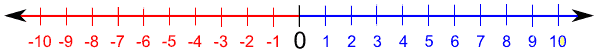
\includegraphics[scale=0.6]{images/integers-numbers-on-number-line.png} 
\caption{The line of integers (image taken from \cite{41}).}
\end{figure}

Then we can describe the action of the element $(0,k)$ on this figure as a shift to the right by $k$ positions, and the element $(1,0)$ as the reflection around the origin($z\longmapsto -z$). Therefore the infinite dihedral group is the group of symmetries of $\Z$, that we represent as a line. 


\subsection{The lamplighter group}
According to \cite{12} the first reference to this algebraic object was anonymously made in \cite{8} in 1983 and remained unnoticed for many years.

\begin{definition}
The \emph{lamplighter group} $\LL$ is the \obs{restricted} wreath product \mbox{$\Z\wr\Z_2=\Z\ltimes\Z_{2}^{(\Z)}$}. 
\end{definition}

The elements of $\LL$ are of the form $(z, (h_{i})_{i\in\Z})$ with $z\in\Z$ and $h_i\in\Z_2$, and just a finite number of $h_i$ are different from $0_{\Z_2}$. Each $(z, (h_{i})_{i\in\Z})$ can be imagined as an infinite dark road ($\Z$), with lampions at every integer ($h_i$), and just a finite number of them turned on (the indices $i$ for which $h_i\neq0_{\Z_2}$). In a specific position $z$, near some lampion, we can see a man, the lamplighter.

\begin{figure}[H]
\begin{center}
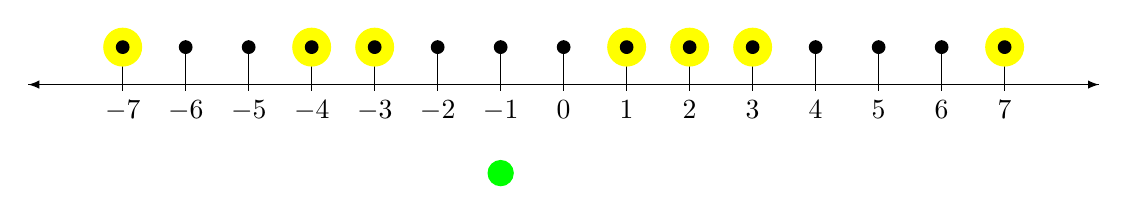
\begin{tikzpicture}[scale=0.8]
\draw[latex-] (-8.5,0) -- (8.5,0) ;
\draw[-latex] (-8.5,0) -- (8.5,0) ;
\foreach \x in  {-7,-6,-5,-4,-3,-2,-1,0,1,2,3,4,5,6,7}
\draw[shift={(\x,0)},color=black] (0cm,0.7cm) -- (0pt,-3pt) node (\x) {};
\foreach \x in {-7,-6,-5,-4,-3,-2,-1,0,1,2,3,4,5,6,7}
\draw[shift={(\x,0)},color=black] (0pt,0pt) -- (0pt,-3pt) node[below] 
{$\x$};

\foreach \x in {-7,-4,-3,1,2,3,7}
\filldraw[color=yellow]([yshift=0.7cm]\x) circle (0.3cm);
\foreach \x in {-7,-6,-5,-4,-3,-2,-1,0,1,2,3,4,5,6,7}
\filldraw[color=black]([yshift=0.7cm]\x) circle (0.1cm);
\filldraw[color=green]([yshift=-1.3cm]-1) circle (0.2cm);
\end{tikzpicture}
\end{center}
\caption{A representation of an \emph{element} $(-1, (h_i)_{i\in\Z})$ in $\LL$. The green circle represent the coordinate $-1$ of the lamplighter, while the yellow circles represent the lit lampions at positions $\{-7,-4,-3,1,2,3,7\}$, i.e., the positions $i$ for which $h_i\neq0_{\Z_2}$.} 
\end{figure}

The product of two elements of $\LL$ is:
$$(z_2, (h_i)_{i\in\Z})*(z_1, (k_i)_{i\in\Z})=(z_1+z_2, (h_{i+z_1} +_{\Z_2} k_i)_{i\in\Z}).$$
The inverse of $(z, (h_{i})_{i\in\Z})$ is $(-z, (h_{i-z})_{i\in\Z_2})$.

\subsection{The adding machine}

\begin{definition}
Let $\abece=\{0,1\}$. The \emph{adding machine} is the synchronous automatic bijective transformation $f=\tau(\id_{\synaut(\abece)},f):\fslovar\longrightarrow\fslovar$, where $\tau$ is the transposition of $\symm(\abece)$.
\end{definition}

We call it adding machine because of the way it acts on $\abece^n$.

\begin{equation}
\begin{split}
f(0y_2\ldots y_n)\:&=\:\tau(0).\id_{\synaut(\abece)}(y_2\ldots y_n)=1y_2\ldots y_n\\
f(1y_2\ldots y_n)\:&=\:\tau(1).f(y_2\ldots y_n)=0.f(y_2\ldots y_n)
\end{split}
\label{eq:add machine def}
\end{equation}


Let us define the function $t_n:\abece^n\longrightarrow\Z/2^n\Z=\Z_{2^n}$ by:
\begin{equation}
t_n(y_1\ldots y_k\ldots y_n)\;=\; y_1+y_22+\cdots+y_{k}2^{k-1}+\cdots+y_n2^{n-1}.
\label{eq:spher}
\end{equation}
It easy to prove that $t_n$ is bijective, and thus we can translate the action of $f$ to $\Z_{2^n}$ by $t_n$.

The equations \eqref{eq:add machine def} tell us that if $x_1\ldots x_k\ldots x_n=\word{w_1}x_k\word{w_2}=\word{w_1}0\word{w_2}$ is a sequence, where $\word{w_1}$ is a sequence of $1$s, while at position $k$ there is the \obs{first element} $x_k=0$, then $f(\word{w_1}x_k\word{w_2})=f(\word{w_1}0\word{w_2})=\word{v_1}.f(0\word{w_2})=\word{v_1}.\tau(0).\id(\word{w_2})=\word{v_1}1\word{w_2}$, where $\word{v_1}$ is a sequence of $0$s. Then \eqref{eq:spher} yields:
\begin{align*}
&(f\circ t_{n}^{-1})  \;	(t_n(x_1\ldots x_k\ldots x_n))=\\
&=(f\circ t_{n}^{-1})  \;	(x_1+x_22+\cdots+x_{k-1}2^{k-2}+x_{k}2^{k-1}+x_{k+1}2^{k}+\cdots+x_n2^{n-1})\\
&=(f\circ t_{n}^{-1}) \;	(1+1\cdot2+\cdots+1\cdot2^{k-2}+0\cdot2^{k-1}+x_{k+1}2^{k}+\cdots+x_n2^{n-1})\\
&=f(1\ldots 10x_{k+1}\ldots x_n)=0\ldots0.f(0x_{k+1}\ldots x_n)=0\ldots0.\tau(0).\id(x_{k+1}\ldots x_n)\\
&=t_{n}^{-1}(0+0\cdot2+\cdots+0\cdot2^{k-2}+ 1\cdot2^{k-1}+ \id(x_{k+1}2^{k}+\cdots+x_n2^{n-1}))\\
&=t_{n}^{-1}(0+0\cdot2+\cdots+0\cdot2^{k-2}+ 1\cdot2^{k-1}+ x_{k+1}2^{k}+\cdots+x_n2^{n-1})\\
&=t_{n}^{-1}(t_n(x_1\ldots x_k\ldots x_n)+1).
\end{align*}

If instead $x_1\ldots x_k\ldots x_n=1\ldots1$ is the sequence without $0$s, we have that:
\begin{align*}
&(f\circ t_n^{-1})  \;	(t_n(x_1\ldots x_k\ldots x_n))=\\
&=(f\circ t_n^{-1}) \;	(1+1\cdot2+\cdots+1\cdot2^{n-1})=(f\circ t_{n}^{-1})(2^n-1)\\
&=f(1\ldots1)=	0\ldots 0=t_{n}^{-1}(0+0\cdot2+\cdots+0\cdot2^{k-2}+ 0\cdot2^{n-1})\\
&=t_{n}^{-1}(1+1\cdot2+\cdots+1\cdot2^{n-1}+1)=t_{n}^{-1}(t_n(x_1\ldots x_k\ldots x_n)+1)=t_{n}^{-1}(2^n)=t_{n}^{-1}(0).
\end{align*}

This means that $t_n\circ f\circ t_{n}^{-1}$ adds 1 to each number in $\Z_{2^n}$. 

Let us now focus on $\langle f\rangle $, the group generated by $f$. In order to study it we need to look closer to a particular property of the function $f$.

\begin{definition}
A left action of $G$ on $X$ is said to be \emph{transitive} if, for each $x,y\in X$, there exists an element $g\in G$ such that $gx=y$.
\end{definition}

\begin{definition}
A synchronous transformation $s:\fslovar\longrightarrow\fslovar$ is called \emph{spherically transitive} if $\langle s\rangle $ acts transitively on $\abece^n$ for each $n$.
\label{def:spherically transitive}
\end{definition}

\begin{proposition}
If a synchronous transformation $s:\fslovar\longrightarrow\fslovar$ is spherically transitive, then $\langle s\rangle $ is infinite.
\end{proposition}
\begin{proof}
Let $n\in\N$ and $\word{w}$ be an element of $\abece^n$. Then, for each $\word{v}\in\abece^n$, there exists $g_{\word{v}}\in \langle s\rangle$ such that $g_{\word{v}}\word{w}=\word{v}$. This yields $|\langle s\rangle|\geqslant n$, so $\langle s\rangle$ is infinite.
\end{proof}

\begin{proposition}
Let $f$ be the adding machine. Then $f$ is spherically transitive and $\langle f\rangle$ is isomorphic to $\Z$.
\end{proposition}
\begin{proof}
Let $\word{y}=y_1y_2\ldots y_n,\:\word{x}=x_1x_2\ldots x_n$ be two sequences in $\abece^n$. As in \eqref{eq:spher} let us consider $t_n(\word{y})$ and $t_n(\word{x})$ in $\Z_{2^n}$. We define $m\in\N\cup\{0\}$ such that $m=t_n(\word{y})-t(\word{x})\;\pmod {2^n}$. Let us consider $f^m\in\langle f\rangle$. Then we have that:
$$t_n(f^m(\word{x}))=t_n(\word{x})+m=t_n(\word{x}) +(t_n(\word{y})-t_n(\word{x}))=t_n(\word{y}) \quad\pmod {2^n} ,$$
which yields $f^m(\word{x})=\word{y}$ because $t_n$ is bijective. Therefore $f$ is spherically transitive and $\langle f\rangle$ is infinite.  We define:
\begin{align*}
\phi:\Z&\longrightarrow  \langle f \rangle\\
m&\longmapsto f^m.
\end{align*}
We have that $ m_1+m_2\mapsto f^{m_1+m_2}=f^{m_1}\circ f^{m_2}$ so $\phi$ is a homomorphism which is obviously surjective. Finally, let $k$ be the smallest element in $\N\cup\{0\}$ such that $\phi(k)=f^0=\id$. If $k\neq 0$ we would have that $|\langle f \rangle|=k$, which is not possible because $\langle f \rangle$ is infinite. Therefore the kernel of $\phi$ is trivial, hence $\phi$ is an isomorphism. 
\end{proof}

We now proceed with the formulation of the theorem.

\smallskip
\subsection{The theorem}

\begin{theorem}\label{th:classification}
Let $\auto{A}=\langle\abece, \QQ, \pi, \lambda\rangle$ be an automaton. Let $\abece=\{0,1\}$ and $|\QQ|=2$. Then the group generated by $\auto{A}$ is isomorphic to one of the following groups:
\begin{enumerate}
\item the trivial group $\{1\}$,
\item the order two group $(\Z_2,+)$,
\item the direct sum $\Z_2\oplus\Z_2$,
\item the infinite cyclic group $\Z$,
\item the infinite dihedral group $\mathcal{D}_\infty$,
\item the lamplighter group $\LL$.
\end{enumerate}
\end{theorem}

I would like to stress the beauty of this theorem, which shows us that also such complex groups as the last three ones can arise from such simple model of machines.

We now provide a part of the proof.

\subsection{Define the cases}
To prove Theorem \autoref{th:classification} we need to examine case by case groups defined by each possible automaton $\auto{A}$. Let us verify in how many ways we can define the functions $\pi$ and $\lambda$.

\begin{itemize}
\item[($\pi$)] Graphically, from each state there exit two possible arrows, and each can arrive to one of the two states. Algebraically, the function $\pi$ has domain $\abece\times\QQ$ and codomain $\QQ$, so for its definition there are $|\QQ|^{|\abece\times\QQ|} = 2^{2\cdot 2} = 16$ possibilities.
\item[($\lambda$)] We can define the output function by its restrictions $\lambda(\cdot,q)$. For each $q\in\QQ$ the function $\lambda(\cdot,q):\abece\longrightarrow\abece$, must be a \obs{permutation} of the alphabet $\abece$. Since $\abece=\{0,1\}$, there are only two possible permutations: the transposition $\tau$, which exchanges the two symbols, and the identity $\id$, which leaves them unchanged. So there are $2$ possibilities for $\lambda(\cdot,q)$ and there are $2$ states $q$ in $\QQ$. This means there are $2\cdot2=4$ possible ways to define $\lambda$. 
\end{itemize}

Overall this means $16\cdot4 = 64$ possible ways to define $\auto{A}$. Let $\{q,s\}$ be the states of the automaton $\auto{A}$. Consequently the group is generated by the actions $a=\LAMBDA_q$ and $b=\LAMBDA_s$. As we have seen in Proposition \autoref{prop:definition of auto by formulas}, we can define $\auto{A}$ by the recursive formulas:
\begin{equation}
\begin{split}
a&=\sigma^{i_1}(x_{11},x_{12}),\\
b&=\sigma^{i_2}(x_{21},x_{22}),
\end{split}
\end{equation}\label{eq: recursive definition}
where $\sigma^{i_1},\sigma^{i_2}$ are elements of $\symm_2:=\symm(\abece)=\symm(\{0,1\})$ and $x_{ij}\in\{a,b\}$ (notice that we have two possibilities for each variable of the equation, so $2^6=64$ cases as seen before). We suppose that $i_1,i_2\in\{0,1\}$ and $\sigma^{0}:=\id_{\symm(2)}$, while $\sigma^1:=\tau$ is the other element of $\symm_2$, the transposition.

\begin{remark}
Recall that $\synaut(\abece)$ acts \emph{faithfully} on $\fslovar$, therefore two elements $c,d$ of $\synaut(\abece)$ act in the same way on $\fslovar$ ($c\word{w}=d\word{w}$ for every $\word{w}$) if and only if $c=d$.
\label{obs: same act=same element}
\end{remark}

\begin{remark}
From now on $\id$ will stand for the identity permutation of some group, usually $\synaut(\abece)$ or $\symm(\abece)$ and it will be clear from the context which specific group is being considered.
\end{remark}

\subsection{Case analysis}

If $\sigma^{i_1}=\sigma^{i_2}=\id_{\symm_2}=\id$, then $a=b=\id_{\synaut(\abece)}$, so we obtain the trivial group $\{1\}$. So we no longer need to consider the 16 cases where
\begin{equation*}
\begin{split}
a&=\id(x_{11},x_{12})=\id,\\
b&=\id(x_{21},x_{22})=\id.
\end{split}
\end{equation*}
We need to consider just the cases where at least one between $\sigma^{i_1}$ and $\sigma^{i_2}$ acts non trivially on $\abece$. We notice that each case:
\begin{equation}\label{eq:focus cases}
\begin{split}
a&=\tau(x_{11},x_{12}),\\
b&=\sigma^{i_2}(x_{21},x_{22}),
\end{split}
\end{equation}
generates the same group as the case:
\begin{equation*}
\begin{split}
a&=\sigma^{i_2}(x_{21},x_{22}),\\
b&=\tau(x_{11},x_{12}).
\end{split}
\end{equation*}
This means that we can analyse just the $2^5=32$ cases (each non-fixed variable has two possible definitions) of the system \eqref{eq:focus cases} to see every possible group generated. 

Let us define $f:\synaut(\abece)\longrightarrow\synaut(\abece)$ by 
\begin{equation}\label{eq:useful homo}
\sigma(c|_0,c|_1)\mapsto\sigma(c|_1,c|_0).
\end{equation}
We have that:
\begin{align*}
f(\gamma(c|_0,c|_1)\sigma(d|_0,d|_1))&=f(\gamma\sigma(c|_{0\sigma}d|_0,c|_{1\sigma}d|_1))=\gamma\sigma(c|_{1\sigma}d|_1,c|_{0\sigma}d|_0))\\
&=\gamma(c|_1,c|_0)\sigma(d|_1,d|_0)
=f(\gamma(c|_0,c|_1))f(\sigma(d|_0,d|_1)),
\end{align*}
so $f$ is a homomorphism. It is easy to verify it is bijective. If $p\in\langle a,b \rangle=G$, then $p=x_1x_2\ldots x_n$ with $x_i\in\{a,b,a^{-1},b^{-1}\}$ and $f(p)=f(x_1x_2\ldots x_n)=f(x_1)f(x_2)\ldots f(x_n)=\in\langle f(a),f(b)\rangle$. This means that $G$ is isomorphic to $f(G)=\langle f(a),f(b)\rangle$. This tells us that the case
\begin{equation*}
\begin{split}
a&=\tau(a,b),\\
b&=\sigma^{i_2}(x_{21},x_{22})
\end{split}
\end{equation*}
generates a group isomorphic to the one generated by the case
\begin{equation*}
\begin{split}
a&=\tau(b,a),\\
b&=\sigma^{i_2}(x_{22},x_{21}).
\end{split}
\end{equation*}
It follows that we can treat only the $24$ cases where $a\in\{\tau(a,a),\tau(a,b),\tau(b,b)\}$.


\subsection{The cases with \texorpdfstring{$a=\tau(a,a)$}{}}

If we have $a=\tau(a,a)=\tau(a|_0,a|_1)$, then:
\begin{equation*}
\begin{split}
a^2 &=\tau(a|_0,a|_1)*\tau(a|_0,a|_1)\\
	&=\tau\tau(a|_{0\tau} a|_0, a|_{1\tau} a_1)\\
	&=\id(a^2,a^2).
\end{split}
\end{equation*}
Therefore $a^2=\id(a^2,a^2)=\id_{\synaut(\abece)}$. This means $a$ acts on $\fslovar$ changing each letter in a word to its opposite ($\abece$ has just two letters), and has order $2$. Now we look at $b$.

\begin{itemize}
\item[(1.1)] If $b=\id(b,b)$, $b=a^2$ acts on $\fslovar$ as the identity, then $\langle a,b\rangle $ is isomorphic to $(\Z_2,+)$ by $a\longmapsto 1$ and $b\longmapsto 0$.
\item[(1.2)] If $b=\tau(a,a)$, then $b=a$ and $\langle a,b\rangle=\langle a\rangle =\{\id,a\}$. Since $a$ has order $2$, $\langle a \rangle$ is isomorphic to $\Z_2$.
\item[(1.3)] If $b=\tau(b,b)$, $b$ acts on $\fslovar$ changing each letter in a word to its opposite, so $b=a$ (recall Remark \autoref{obs: same act=same element}) and so $\langle a,b\rangle =\langle a \rangle$ is again isomorphic to $\Z_2$.
\item[(1.4)] If $b=\id(a,a)$, then $b$ acts on $\fslovar$ by changing each letter but the first one, so $b^2=\id_{\synaut(\abece)}$. Furthermore, $ab$ acts by changing just the first letter, and the same does $ba$, so recalling Remark \autoref{obs: same act=same element}, since they acts in the same way on $\fslovar$, $ba=ab$. It follows that $\langle a,b\rangle =\{\id=a^2,a,b,ab\}$ is isomorphic to $(\Z_2\oplus\Z_2, +)$ by the maps
\begin{align*}
a^2=b^2&\longmapsto (0,0),\\
a&\longmapsto (1,1),\\
b&\longmapsto (0,1),\\
ab=ba&\longmapsto (1,0).
\end{align*}
\item[(1.5)] If $b=\tau(a,b)=\tau(b|_0,b|_1)$ then: 
$$ba^{-1}=ba=\tau(a,b)\tau(a,a)=\tau\tau(ba,aa)=\id(ba,aa)=\id_{\symm_2}(ba,\id_{\synaut(\abece)}).$$
Therefore, $ba$ acts by leaving the first letter unchanged, and if the second letter is $0$ acts again, otherwise $a^2=\id_{\synaut(\abece)}$ acts on the rest of the word. So $ba$ leaves each word unchanged: $ba=\id$. So $b=a^{-1}=a$, because $a$ has order $2$. So again we have an isomorphism to $\Z_2$.
\item[(1.6)] If $b=\id(a,b)$ we obtain the infinite dihedral group. The proof is omitted.
\item[(1.7)] If $b=\tau(b,a)$, with the homomorphism $f$ defined in \eqref{eq:useful homo}, we have that $\langle a,b \rangle=\langle \tau(a,a),\tau(b,a) \rangle$ is isomorphic to the group of case (1.5) $\langle f(a),f(b) \rangle=\langle \tau(a,a),\tau(a,b) \rangle$.
\item[(1.8)] If $b=\id(b,a)$ the group $\langle a,b \rangle=\langle \tau(a,a),\id(b,a) \rangle$ is isomorphic to $\langle f(a),f(b) \rangle=\langle \tau(a,a),\id(a,b) \rangle$, i.e., case (1.6).
\end{itemize}

\subsection{The cases with \texorpdfstring{$a=\tau(b,a)$}{}}

Let $a=\tau(b,a)=\tau(a|_0,a|_1)$.
\begin{itemize}
\item[(2.1)] If $b=\tau(b,a)=\tau(b|_0,b|_1)$ then $a=b$, therefore $a=\tau(a,a)=b=\tau(a,a)$ and so $\langle a,b\rangle $, as in case (1.2), is isomorphic to $\Z_2$.
\item[(2.2)] If $b=\tau(a,b)=\tau(b|_0,b|_1)$ then
\begin{align*}
 ba^{-1}&=	\:\tau(b|_0,b|_1)\:\tau(a|_1^{-1},a|_0^{-1})=	\tau\tau(b|_1a|_1^{-1},b|_0a|_0^{-1})\\
		&=\id(ba^{-1},ab^{-1}),\\
 ab^{-1}&=	\:\tau(a|_0,a|_1)\tau(b|_1^{-1},b|_0^{-1})=	\:\id(a|_1b|_1^{-1},a|_0b|_0^{-1})\\
 		&=\id(ab^{-1},ba^{-1}).
\end{align*}
This yields that if $c:=ba^{-1}$ and $d:=ab^{-1}$, then
\begin{align*}
 c=\id(c,d),\\
 d=\id(d,c).
\end{align*}
So $c=d=\id_{\synaut(\abece)}$, because they both leave each word unchanged. This gives us the equality $\id_{\synaut(\abece)}=c=ba^{-1}$ which leads to $a=b=\tau(a,b)=\tau(b,b)$, and consequently to $a^2=\id(a^2,a^2)=\id_{\synaut(\abece)}$. So $\langle a,b\rangle =\langle a\rangle =\{\id_{\synaut(\abece)},a\}$, which is isomorphic to $\Z_2$.
\item[(2.3)] If $b=\tau(b,b)$, then denoting $b':=a$ and $a':=b$, we get $a'=\tau(a',a')$ and $b'=\tau(a',b')$ and we see again the case (1.5), so isomorphism with $\Z_2$.
\item[(2.4)] If $b=\tau(a,a)$ we have:
\begin{align*}
 ba^{-1}&=\;\tau(a,a)\tau(a^{-1},b^{-1})\:=\:\id(\id,ab^{-1}),\\
 ab^{-1}&=\;\tau(b,a)\tau(a^{-1},a^{-1})\:=\:\id(\id,ba^{-1}).
\end{align*}
Then defining $c:=ba^{-1}$ and $d:=ab^{-1}$, we get the same conclusion as in case (2.2), isomorphism with $\Z_2$.
\item[(2.5)] If $b=\id(b,b)$, then $b=\id_{\synaut(\abece)}$, and $a=\tau(\id_{\synaut(\abece)},a)$. Here $a$ acts as the adding machine. Therefore $\langle a,b\rangle =\langle a\rangle $ is isomorphic to $\Z$.
\item[(2.6)] If $b=\id(a,a)$, the group $G:=\langle a,b\rangle $ is isomorphic to $\Z$. To arrive to this result we shall prove that $G$ is cyclic, i.e., is generated by one element. We omit the proof that its cardinality is infinite. Then $G$, being infinite and cyclic, it is isomorphic to $\Z$. We prove that $G$ is cyclic:
\begin{align*}
ba&=\id(a,a)\tau(b,a)=\tau(ab,a^2),\\
ab&=\tau(b,a)\id(a,a)=\tau(ba,a^2),
\end{align*}
which yields $ba=ab$, that is $\langle a,b\rangle $ is abelian. Furthermore,
$$ba^2=ba\:a=\tau(ba,a^2)\tau(b,a)=\id(a^2b,a^2b).$$
Consequently, $ba^2=1$. We claim that $G:=\langle a,b\rangle =\langle ab\rangle $. In fact $ab$ generates $b$ by $(ab)^2=abab=b(ba^2)=b$, and $ab$ and $b$ generate $a$ by $abb^{-1}=a$. Therefore $G$ is cyclic generated by $ab$.

\item[(2.7)] If $b=\id(b,a)$ then $\langle a,b\rangle =\LL$ is the lamplighter group $\LL$, but we are going to skip the proof.

\item[(2.8)] If $b=\id(a,b)$, we can reach the symmetric case of the (2.7). Let us take $b^{-1}=\id(a^{-1},b^{-1})\;,\;a^{-1}=\tau(a^{-1},b^{-1})$. In general, since $a^{-1},b^{-1}\:\in\:\langle a,b\rangle $, and consequently $a,b\:\in\:\langle a^{-1},b^{-1}\rangle $, we have that $\langle a,b\rangle \:=\:\langle a^{-1},b^{-1}\rangle $. So we can observe the group generated by $a^{-1},b^{-1}$. Let us now take a generic element $d=\tau(d,d)\in\synaut(\abece)$. Then:
\begin{align*}\label{eq:case2.8}
(b^{-1})^d\:=d^{-1}b^{-1}d&=\tau(d^{-1},d^{-1})\:\id(a^{-1},b^{-1})\:\tau(d,d)=\id((b^{-1})^d,(a^{-1})^d),\\
(a^{-1})^d\:=d^{-1}a^{-1}d&=\tau(d^{-1},d^{-1})\:\tau(a^{-1},b^{-1})\:\tau(d,d)=\tau((b^{-1})^d,(a^{-1})^d).
\end{align*}
Let us call $b':=\:b^{-1}$ and $a'=a^{-1}$. We showed that we can study the group generated by $a',b'$. Let us take the generic element $x_1x_2\ldots x_k$ with $x_i\in\{a',b'\}$. We observe that its conjugate by $d$, $(x_1x_2\ldots x_k)^d$, is the same as $(x_1)^d(x_2)^d\ldots (x_k)^d$. This tells us that the each element in $\langle a'^d,b'^d\rangle $ is conjugate to some element of $\langle a',b'\rangle $ and viceversa. So the conjugate of the group $\langle a',b'\rangle $ is $\langle a'^d,b'^d\rangle $, therefore they are isomorphic.
So again, with another jump, we can define $b'':=(b^{-1})^d=b'^d$ and $a'':=(a^{-1})^d=a'^d$ and focus on $\langle a'',b''\rangle $ that is isomorphic to $\langle a,b\rangle $. For the equations above we have that:
\begin{align*}
a''&=\tau(b'',a''),\\
b''&=\id(b'',a'').
\end{align*}
That is the case (2.7).
\end{itemize}


\subsection{The cases with \texorpdfstring{$a=\tau(b,b)$}{}}

Let $a=\tau(b,b)$.
\begin{itemize}
\item[(3.1)-(3.2)] The case $b=\tau(a,b)$ is analogous to (2.4), while the case $b=\tau(b,a)$ is symmetrical to (2.4), both leading to $\Z_2$.
\item[(3.3)-(3.4)] If $b=\tau(b,b)$ then $b=a=\tau(a,a)$, and we have the case (1.2) with $\Z_2$. If $b=\tau(a,a)$ we arrive to the same conclusion.
\item[(3.5)] If $b=(b,b)$ then $b=\id$ and $a=\tau(\id,\id)$, so $\langle a\rangle =\{\id,a\}$ is isomorphic to $\Z_2$.
\item[(3.6)-(3.7)] These cases lead to the infinite dihedral group. The proof is omitted.
\item[(3.8)] If $b=\id(a,a)$, then:
\begin{align*}
a^2&=\id(b^2,b^2),\\
b^2&=\id(a^2,a^2),\\
 ba&=\tau(ab,ab),\\
 ab&=\tau(ba,ba).
\end{align*}
This yields $a^2=b^2=\id$ and to $ab=ba=\tau(ab,ab)$ (abelian group). For this reason we can see each possible word $x_1x_2\ldots x_k$ with $x_i\in\{a,b,a^{-1},b^{-1}\}=\{a,b\}$ as $a^nb^m$ where $n+m=k$. In addition, we know that $a^n=a^{n\;\pmod 2}$ and $b^m=b^{m\;\pmod 2}$, so each possible composition of $a$ and $b$ is an element $a^ib^j$, where $i,j\in\{0,1\}$. So the group $\langle a,b\rangle =\{\id,a,b,ab\}$ is isomorphic to $\Z_2\oplus\Z_2$ by:
\begin{align*}
\id&\longmapsto (0,0),\\
a&\longmapsto (1,0),\\
b&\longmapsto (0,1),\\
ba&\longmapsto (1,1). 
\end{align*}\qed
\end{itemize}



\bigskip
\appendix
\section*{Concluding remarks}

In this thesis we have gone through just a part of the theory of automata. We considered just finite deterministic Mealy automata, but if instead the reader may want to explore a broader class of objects, \cite{4} is a very good source where to start from. Otherwise for some more practical application of the theory there is the book \cite{11}. The book \cite{9} explores in the details the structures of Subsection \ref{subsec:wreath prod}.

If the reader is interested to know more about the lamplighter group, I can recommend \cite{1} for an approach which requires just the knowledge of an undergraduate, and \cite{12} for an analysis in the case we take a finite version of this object. 

For more examples of automata in connection to groups I recommend \cite{2}, where the complete classification of 3-state automata over a 2-letter-alphabet can be found. The book \cite{10} is another very good source, and the article \cite{13} shows some important algebraic problems which can be solved with the group generated by some specific automaton. The most notable example in the latter class is the first Grigorchuk group, analysed in 1984 in \cite{6}.

\section*{Acknowledgements}
I would like to thank both my Supervisors prof.\ Alessandro Logar and izr.\ prof.\ Ganna Kudryavtseva, and in particular the latter one, for all the time she spent helping me and for her infinite patience with my clumsiness. Then I would like to thank prof.\ Valentina Beorchia and prof.\ Marko Petkovšek thanks to whom I could participate in this exchange program. Without them this would not have even started. I need to thank also prof.\ Sašo Strle, who managed to follow me and other tens of students in the completion of the bachelor thesis, and the administrative offices of Ljubljana and Trieste, which helped me with the bureaucracy. Remarkably important was the assistance of my dear friend and collegue Matej Jazbec, who corrected my slovenian translations. Finally I would like to thank my beloved ones, who managed to bear me during the last period.


\bigskip
\begin{thebibliography}{99}
%how to write bibliography:
%alphabetic order

%Every work must be cited at least once
%A.~B.~LastName
%and before the last author (if more than one)
%general format for books:
%Authors, \emph{Title}, Collection, Publisher, City, Year.
%
%If a part of collection: 
%in: Title (Ed. Editor/Eds. Editors)
%
%Science \textbf{215} (1999) 325--327,
%
%similar for other journal entries 

\bibitem{1} M. C. ~Bonanome, M. H. ~Dean and J. P. ~Dean, \emph{A sampling of remarkable groups}, Thompson, self-similar, lamplighter and Baumslag-solitar, Compact Textbooks in Mathematics, Birkhäuser Springer, Cham, 2018.

\bibitem{2} I. ~Bondarenko, R. ~Grigorchuk, R. ~Kravchenko, Y. ~Muntyan, V. ~Nekrashevych, D. ~Savchuk and Z. ~Sunic, \emph{On classification of groups generated by 3-state automata over a 2-letter alphabet}, Algebra Discrete Math. \textbf{1} (2008) 1--163.

\bibitem{Doote} D. S. Dummit and R. M. Foote, \textit{Abstract algebra}, 3rd ed., Wiley, Chichester, 2003.

\bibitem{4} S. ~Eilenberg, \emph{Automata, language, and machines}, Vol. A, Pure and Applied Mathematics \textbf{59}, Academic Press, New York, 1974.

\bibitem{6} R. I. ~Grigorchuk and A. ~Machí, \textit{An example of an indexed language of intermediate growth}, Theor. Comput. Sci. \textbf{215} (1999) 325--327.

\bibitem{5} R. I. ~Grigorchuk, V. V. ~Nekrashevych and V. V. ~Sushchanskiix, \emph{Automata, dynamical systems, and groups}, Proc. Steklov Inst. Math. \textbf{231} (2000) 128--203.

\bibitem{7} R. I. ~Grigorchuk and A. ~Żuk, \textit{The lamplighter group as a group generated by a 2-state automaton, and its spectrum}, Geom. Dedicata \textbf{87} (2001) 209--244.

\bibitem{8} V. A. ~Kaimanovich and A. M. ~Vershik, \emph{Random walks on discrete groups: boundary and entropy}, Ann. Probab. \textbf{11} (1983) 457--490.

\bibitem{9} J. D. P. ~Meldrum, \emph{Wreath products of groups and semigroups}, Pitman Monographs and Surveys in Pure and Applied Mathematics \textbf{74}, Longman/Wiley, Harlow, 1995.

\bibitem{10} V. V. Nekrashevych, \emph{Self-similar groups}, Mathematical Surveys and Monographs \textbf{117}, Amer. Math. Soc., Providence, 2005.

\bibitem{11} J. ~Rhodes, \emph{Applications of automata theory and algebra}, Via the mathematical theory of complexity to biology, physics, psychology, philosophy and games, World Scientific Publishing Co. Pte. Ltd., Singapore, 2009.

\bibitem{12} J. A. ~Siehler, \emph{The finite lamplighter groups: a guided tour}, College Math. J. \textbf{43} (2012) 203--211.

\bibitem{13} A. Zuk, \textit{Automata groups}, in: Topics in non-commutative geometry, Clay Math. Proc. \textbf{16}, Amer. Math. Soc., Providence, 2012, pp 165--196.

\bibitem{41} The line of integers, available at \url{https://www.math-only-math.com/images/integers-numbers-on-number-line.png}, [viewed 21. 03. 2021].

\end{thebibliography}

\end{document}

